%%%%%%%%%%%%%%%%%%%%%%%%%%%%%%%%%%%%%%%%%%%%%%%%%%%%%%%%%%%%%%%%%%%%%%%%%%%%%%%%%%%
%%  This template is created by Philipp Ludewig	and its based on the       	     %%
%%  MES template by Jan Boelmann and Shashi Kiran ShivarKumar Honnali			 %%
%%  for further informations please contact: [postkasten@zphilippludewig.de]     %%
%%																			     %%
%%																			   	 %%
%%																			     %%
%% 																			     %%
%%                                                                		         %%
%%%%%%%%%%%%%%%%%%%%%%%%%%%%%%%%%%%%%%%%%%%%%%%%%%%%%%%%%%%%%%%%%%%%%%%%%%%%%%%%%%%

%%%%%%%%%%%%%%%%%%%%%%%%%%%%%%%%%%%%%%%%%%%%%%%%%%%%%%%%%%%%%%%%%%%%%%%%%%%%%%%%%%%
%%%%   						     Arara	                                       %%%%
%%%%%%%%%%%%%%%%%%%%%%%%%%%%%%%%%%%%%%%%%%%%%%%%%%%%%%%%%%%%%%%%%%%%%%%%%%%%%%%%%%%       
%% hier wird der Ablauf des Automatisierungstools definiert			             %%
%%%%%%%%%%%%%%%%%%%%%%%%%%%%%%%%%%%%%%%%%%%%%%%%%%%%%%%%%%%%%%%%%%%%%%%%%%%%%%%%%%%
% arara: pdflatex  { action: nonstopmode, shell: on }
% arara: pdflatex  { action: nonstopmode, shell: on }
% arara: biber
% arara: pdflatex  { action: nonstopmode, shell: on }
% arara: pdflatex  { action: nonstopmode, shell: on }
% arara: clean: { files: [ Index.aux, Index.bbl ] }
% arara: clean: { files: [ Index.bcf, Index.cod ] } 
% arara: clean: { files: [ Index.blg, Index.lof ] }
% arara: clean: { files: [ Index.lot, Index.out ] } 
% arara: clean: { files: [ Index.toc, Index.log ] } 
% arara: clean: { files: [ Index.run.xml ] }

%%%%%%%%%%%%%%%%%%%%%%%%%%%%%%%%%%%%%%%%%%%%%%%%%%%%%%%%%%%%%%%%%%%%%%%%%%%%%%%%%%%
%%%%   						     Preamble                                      %%%%
%%%%%%%%%%%%%%%%%%%%%%%%%%%%%%%%%%%%%%%%%%%%%%%%%%%%%%%%%%%%%%%%%%%%%%%%%%%%%%%%%%%       
%% hier wird das Dokument mit den Einstellungen von oben definiert               %%
%%%%%%%%%%%%%%%%%%%%%%%%%%%%%%%%%%%%%%%%%%%%%%%%%%%%%%%%%%%%%%%%%%%%%%%%%%%%%%%%%%%

\documentclass[
   13pt,               % Schriftgroesse 13pt
   a4paper,             % Layout fuer Din A4
   oneside,             % Layout fuer einseitigen Druck
   headinclude,         % Kopfzeile wird Seiten-Layouts mit beruecksichtigt
   headsepline,         % horizontale Linie unter Kolumnentitel
%  footinclude,         % Kopfzeile wird Seiten-Layouts mit beruecksichtigt
%  footsepline,         % horizontale Linie unter Kolumnentitel
%  plainheadsepline,    % horizontale Linie auch beim plain-Style
   plainfootsepline,    % horizontale Linie auch beim plain-Style
   BCOR12mm,            % Korrektur fuer die Bindung
   DIV18,               % DIV-Wert fuer die Erstellung des Satzspiegels, siehe scrguide
%  halfparskip,         % Absatzabstand statt Absatzeinzug
   openany,             % Kapitel können auf geraden und ungeraden Seiten beginnen
   bibliography=totoc,            % Literaturverz. wird ins Inhaltsverzeichnis eingetragen
   listof=totoc,				% Abbildungs und TabellenVZ ins InhaltsVZ
%  pointlessnumbers,    % Kapitelnummern immer ohne Punkt
   numbers=noenddot,
   %tablecaptionabove,   % korrekte Abstaende bei TabellenUEBERschriften
   fleqn,               % fleqn: Glgen links (statt mittig)
   %draft               % Keine Bilder in der Anzeige, overfull hboxes werden angezeigt
   xcolor=table
]{scrbook}

%%%%%%%%%%%%%%%%%%%%%%%%%%%%%%%%%%%%%%%%%%%%%%%%%%%%%%%%%%%%%%%%%%%%%%%%%%%%%%%%%
%%%%% 					     Einstellungen	      							%%%%%
%%%%%%%%%%%%%%%%%%%%%%%%%%%%%%%%%%%%%%%%%%%%%%%%%%%%%%%%%%%%%%%%%%%%%%%%%%%%%%%%%

%% Dadurch werden die Parameter der Vorlage wie Schriftart, Größe usw. geladen.
%% Der Befehl "\input{file} lädt eine Datei, ohne sie im Dokument anzuzeigen.
% Alle Pakete um dieses Latex Dokument zu erweitern

%%%%%%%%%%%%%%%%%%%%%%%%%%%%%%%%%%%%%%%%%%%%%%%%%%%%%%%%%%%%%%%%%%%%%%%%%%%%%%%%%%%
%%%%   						     Packages                                      %%%%
%%%%%%%%%%%%%%%%%%%%%%%%%%%%%%%%%%%%%%%%%%%%%%%%%%%%%%%%%%%%%%%%%%%%%%%%%%%%%%%%%%%       
%% hier werden die verwendeten Pakete und ihre Optionen definiert. 				 %%
%% die Veränderung der Reihenfolge wie die Pakete definiert sind wird abgeraten  %%
%%%%%%%%%%%%%%%%%%%%%%%%%%%%%%%%%%%%%%%%%%%%%%%%%%%%%%%%%%%%%%%%%%%%%%%%%%%%%%%%%%%
\usepackage{graphicx} 					% Required to insert images
\usepackage{longtable}					% Required for tables over several pages
\usepackage{lscape}	
\usepackage{floatrow}					% Required to place several images side by side
\usepackage{listings}					% Required for insertion of code
\usepackage{courier} 					% Required for the courier font
\usepackage[ngerman]{babel} % Required for german language
\RequirePackage[ngerman=ngerman-x-latest]{hyphsubst} % Required for correct wrapping of Words
\usepackage[utf8]{inputenc} % Required for UTF-8 based vowels like äöü
\usepackage[T1]{fontenc} % Required for UTF-8 Fonts
\usepackage[hyphens]{url} % Required for placing URL in Text

%% BibLaTeX-settings: (see biblatex reference for further description)
\newcommand{\mybiblatexstyle}{authoryear}

\newcommand{\mybiblatexdashed}{false}  %% "true" or "false"
%% If true: replace recurring reference authors with a dash.

\newcommand{\mybiblatexbackref}{true}  %% "true" or "false"
%% If true: create backward links from reference to citations.
\usepackage[
backend=biber, 		%% using "biber" to compile references (instead of "biblatex")
style=\mybiblatexstyle, 		%% see biblatex documentation
citestyle=numeric,			%% see biblatex documentation
sortlocale=de_DE,				%% see biblatex documentation
dashed=\mybiblatexdashed, 		%% do *not* replace recurring reference authors with a dash
backref=\mybiblatexbackref, 	%% create backlings from references to citations
natbib=true, 					%% offering natbib-compatible commands
hyperref=auto, 					%% using hyperref-package references
url=true, 
doi=true,
eprint=false
]{biblatex}  					%% remove, if using BibTeX instead of biblatex
\usepackage{bibgerm} % Required for german 	bibliography style
\usepackage{wrapfig} % Required for picture which are surrended by text
\usepackage{float} % Required for floating pictures in text
\usepackage{microtype} % For smaller Text http://www.khirevich.com/latex/microtype/



\usepackage[usenames,dvipsnames]{xcolor} % Required for coloring text
\usepackage{colortbl} % Required for coloring tables
\usepackage{booktabs} % Required for indivduell horizontal lines in a table

%\usepackage[square,sort,comma,numbers]{natbib} % Required for Bibliographystyles like dinat
\usepackage{lmodern} % Required to change the style of the text

\usepackage{eurosym} % Required to write €

\usepackage{fancyhdr} % For Pagestyle
\usepackage[onehalfspacing]{setspace} % Required to change linepitch

\usepackage[font=footnotesize]{caption} % Required for captions under tables and pictures

\usepackage{hyperref} % Package for hyperref
\hypersetup{
	colorlinks=true, %Colours links instead of ugly boxes
	urlcolor=blue, %Colour for external hyperlinks
	linkcolor=blue, %Colour of internal links
	citecolor=blue %Colour of citations, could be ``red''
}

\usepackage{lipsum} % Required for filling sections with nonsense text. 
\usepackage{textcomp} % Required for text symbols
\usepackage{acronym}  % Required for Glossar
\usepackage{pifont} 			%% For additional special characters available by \verb#\ding{}#
\usepackage{mathtools} % Required for math stuff
\usepackage{verbatim} % Required for writing Latex Code as Text
\usepackage{paralist} % Required for special lists
\usepackage{pdfpages} % Required for including PDF Pages

\usepackage{accsupp}
\newcommand*{\noaccsupp}[1]{\BeginAccSupp{ActualText={}}#1\EndAccSupp{}}
\usepackage[fencedCode,inlineFootnotes,citations,definitionLists,hashEnumerators,smartEllipses,hybrid]{markdown} % Required for writing in markdown syntax
% Not in Use
% \usepackage{titlesec}
% \usepackage{mdframed}
% \usepackage{calc}
% \usepackage{colortbl}
%\usepackage[scaled]{uarial}
% \usepackage{lastpage} 					% Required to determine the last page for the footer
% \usepackage{extramarks} 	 			% Required for headers and footers


% Sämtliche Metadaten
\newcommand{\sArtofExam}{Leistungsnachweis } % oder Bachelor-Thesis oder Master-Thesis oder Protokoll etc.
\newcommand{\sName}{Hans im Glück}
\newcommand{\sMtrNr}{98654}
\newcommand{\sFirstTutor}{Prof. Dr. Einstein}
\newcommand{\sSecondTutor}{Prof. Dr. Düsentrieb}
\newcommand{\sTitle}{Einfacher Leistungsnachweise schreiben mit LaTeX}
\newcommand{\sCaption}{Latex-Vorlage für Anfänger und Fortgeschrittene}
\newcommand{\TitleDescription}{Latex Vorlage für Bachelor- und Master}
\newcommand{\sModul}{Modules}
\newcommand{\sCompany}{DuckTales AG}
\newcommand{\sDegree}{Bachelor}
\newcommand{\sFaculty}{Wirtschaftsinformatik / Informatik}
\newcommand{\sDepartment}{Fachbereich 2 }
\newcommand{\sUni}{Hochschule Bremerhaven}
\newcommand{\sLocation}{Bremerhaven}
\newcommand{\sTime}{April 2017}
\newcommand{\sVersion}{version 0.1}
\newcommand{\sSubmissiondate}{2. April 2017}




% Einstellungen zu den Farben
%============= Eigene Farben ==============

\definecolor{mygreen}{rgb}{0,0.6,0}
\definecolor{mygray}{rgb}{0.5,0.5,0.5}
\definecolor{mymauve}{rgb}{0.58,0,0.82}
\definecolor{DarkGrey}{rgb}{0.1,0.1,0.1}
\definecolor{TitleBox}{RGB}{177,177,237}
\definecolor{DocumentLinkColor}{rgb}{0,0,0}
\definecolor{background}{HTML}{eeeeee}
\definecolor{delim}{RGB}{20,105,176}
\colorlet{numb}{magenta!60!black}
\colorlet{punct}{red!60!black}

%===========================================

%=========== Styles for Coding =============
\lstdefinestyle{CodeBox} {
	language=C,
    basicstyle=\footnotesize\ttfamily,
    numbers=left,
%     numberstyle=\scriptsize,
    stepnumber=2,
    numbersep=8pt,
    showstringspaces=false,
    breaklines=true,
    frame=lines,
    tabsize=2,
    backgroundcolor=\color{background},
    breakatwhitespace=false,
	breaklines=true,
	commentstyle=\color{mygreen},
	deletekeywords={...},
	keepspaces=true,
	keywordstyle=\color{blue},
	morekeywords={*,...},
	numbers=left,
	numberstyle=\tiny\color{mygray},
	showspaces=false,
	showtabs=false,
	stringstyle=\color{mymauve}
}

\lstdefinestyle{ps1} {
	backgroundcolor=\color{white},   	% choose the background color; you must add \usepackage{color} or \usepackage{xcolor}
	basicstyle=\footnotesize\ttfamily, 	% the size of the fonts that are used for the code
	breakatwhitespace=false,        	% sets if automatic breaks should only happen at whitespace
	breaklines=true,               		% sets automatic line breaking
	commentstyle=\color{black},    		% comment style
	deletekeywords={...},            	% if you want to delete keywords from the given language
	escapeinside={\%*}{*)},          	% if you want to add LaTeX within your code
	extendedchars=true,              	% lets you use non-ASCII characters; for 8-bits encodings only, does not work with UTF-8
	frame=none,                  		% adds a frame-border to the bottom
	keepspaces=true,                 	% keeps spaces in text, useful for keeping indentation of code (possibly needs columns=flexible)
	keywordstyle=\color{black},       	% keyword style
	language=bash, 	                	% the language of the code
	morekeywords={*,...},            	% if you want to add more keywords to the set
	numbers=none,                    	% where to put the line-numbers; possible values are (none, left, right)
	showspaces=false,               	% show spaces everywhere adding particular underscores; it overrides 'showstringspaces'
	showstringspaces=false,          	% underline spaces within strings only
	showtabs=false,                  	% show tabs within strings adding particular underscores
	stringstyle=\color{black},     		% string literal style
	tabsize=4	                      	% sets default tabsize to 2 spaces
}

\lstdefinestyle{json}{
    basicstyle=\footnotesize\ttfamily,
    numbers=left,
    numberstyle=\scriptsize,
    stepnumber=2,
    numbersep=8pt,
    showstringspaces=false,
    breaklines=true,
    frame=lines,
    deletekeywords={...},
    backgroundcolor=\color{background},
    tabsize=2,
    literate=
     *{0}{{{\color{numb}0}}}{1}
      {1}{{{\color{numb}1}}}{1}
      {2}{{{\color{numb}2}}}{1}
      {3}{{{\color{numb}3}}}{1}
      {4}{{{\color{numb}4}}}{1}
      {5}{{{\color{numb}5}}}{1}
      {6}{{{\color{numb}6}}}{1}
      {7}{{{\color{numb}7}}}{1}
      {8}{{{\color{numb}8}}}{1}
      {9}{{{\color{numb}9}}}{1}
      {:}{{{\color{punct}{:}}}}{1}
      {,}{{{\color{punct}{,}}}}{1}
      {\{}{{{\color{delim}{\{}}}}{1}
      {\}}{{{\color{delim}{\}}}}}{1}
      {[}{{{\color{delim}{[}}}}{1}
      {]}{{{\color{delim}{]}}}}{1},
}

\lstdefinestyle{LaTeX}
{
	language={[LaTeX]TeX},
	alsolanguage={PSTricks},
	numbersep=1em,
	numberstyle=\tiny\color{red}\noaccsupp,
	xleftmargin=\dimexpr\fboxsep+\fboxrule\relax,
	xrightmargin=\dimexpr\fboxsep+\fboxrule\relax,
	breaklines=true,
	basicstyle=\small\tt,
	keywordstyle=\color{blue},
	commentstyle=\color[rgb]{0.13,0.54,0.13},
	backgroundcolor=\color{yellow!10},
	tabsize=2,
	columns=flexible,
	morekeywords={
		graphicspath,
		includegraphics,
		blinddocument,
	},
}

\lstdefinestyle{Bash}
{	language=Bash,
	backgroundcolor=\color{DarkGrey},
	keywordstyle=\color{BlueViolet}\bfseries,
	commentstyle=\color{Grey},
	stringstyle=\color{Red},
	showstringspaces=false,
	basicstyle=\small\color{white},
	numbers=none,
	captionpos=b,
	tabsize=4,
	breaklines=true
}
%===========================================

%=========== Character for UTF-8 ===========

\lstset{literate=
	{á}{{\'a}}1 {é}{{\'e}}1 {í}{{\'i}}1 {ó}{{\'o}}1 {ú}{{\'u}}1
	{Á}{{\'A}}1 {É}{{\'E}}1 {Í}{{\'I}}1 {Ó}{{\'O}}1 {Ú}{{\'U}}1
	{à}{{\`a}}1 {è}{{\`e}}1 {ì}{{\`i}}1 {ò}{{\`o}}1 {ù}{{\`u}}1
	{À}{{\`A}}1 {È}{{\'E}}1 {Ì}{{\`I}}1 {Ò}{{\`O}}1 {Ù}{{\`U}}1
	{ä}{{\"a}}1 {ë}{{\"e}}1 {ï}{{\"i}}1 {ö}{{\"o}}1 {ü}{{\"u}}1
	{Ä}{{\"A}}1 {Ë}{{\"E}}1 {Ï}{{\"I}}1 {Ö}{{\"O}}1 {Ü}{{\"U}}1
	{â}{{\^a}}1 {ê}{{\^e}}1 {î}{{\^i}}1 {ô}{{\^o}}1 {û}{{\^u}}1
	{Â}{{\^A}}1 {Ê}{{\^E}}1 {Î}{{\^I}}1 {Ô}{{\^O}}1 {Û}{{\^U}}1
	{œ}{{\oe}}1 {Œ}{{\OE}}1 {æ}{{\ae}}1 {Æ}{{\AE}}1 {ß}{{\ss}}1
	{ű}{{\H{u}}}1 {Ű}{{\H{U}}}1 {ő}{{\H{o}}}1 {Ő}{{\H{O}}}1
	{ç}{{\c c}}1 {Ç}{{\c C}}1 {ø}{{\o}}1 {å}{{\r a}}1 {Å}{{\r A}}1
	{€}{{\euro}}1 {£}{{\pounds}}1 {«}{{\guillemotleft}}1
	{»}{{\guillemotright}}1 {ñ}{{\~n}}1 {Ñ}{{\~N}}1 {¿}{{?`}}1
}

% \lstset{style=CodeBox}
\DeclareCaptionFont{white}{\color{white}}
% \DeclareCaptionFormat{listing}{\colorbox{TitleBox}{\parbox{\fboxsep}{#1#2#3}}}
\DeclareCaptionFormat{listing}{\colorbox{TitleBox}{\parbox{\dimexpr\textwidth-2\fboxsep\relax}{#1#2#3}}}
\captionsetup[lstlisting] {
	format=listing,
	font={sf}
}

% Einstellungen zu den Seiten
\pagestyle{fancy} %eigener Seitenstil
\fancyhf{} %alle Kopf- und Fußzeilenfelder bereinigen
\fancyhead[L]{} %Kopfzeile links
\fancyhead[C]{} %zentrierte Kopfzeile
\fancyhead[R]{} %Kopfzeile rechts
\renewcommand{\headrulewidth}{1.0pt} %obere Trennlinie
\fancyfoot[C]{\thepage} %Seitennummer
\renewcommand{\footrulewidth}{1.0pt} %untere Trennlinie

%\pagestyle{scrheadings}
%\ihead[]{\headmark}
%\chead[]{}
%\ohead[]{}
%\ifoot[]{}
%\cfoot[]{}
%\ofoot[\pagemark]{\pagemark}
%\setheadsepline{1.0pt}
%\setfootsepline{1.0pt}

\hypersetup{
	breaklinks = {true}, %Erlaubt Zeilenumbrüche in Links
	colorlinks = {true}, %Benutze farbige Links
	citecolor = {DocumentLinkColor}, %Farbe für Zitate
	linkcolor = {DocumentLinkColor}, %beeinflusst Inhaltsverzeichnis und Seitenzahlen
	urlcolor = {DocumentLinkColor}, %Weblink-Farbe
	pdftitle = {Konzeption und Entwicklung eines hochverfügbaren VPN-Clusters auf Basis von Debian Linux}, %Titel der Arbeit
	pdfsubject = {Bachelor-Thesis}, %Thema der Arbeit
	pdfauthor = {Jan Torben Bein}, %AutorIN der Arbeit
	pdfkeywords = {Cluster HA Linux Debian OpenVPN VPN Corosync Pacemaker Heartbeat}, %Stichwörter zur Arbeit
	pdfproducer = {pdfLaTeX}, %Erzeugt durch
	pdfcreator = {MiKTeX}, %Erstellt mit
	pdfstartview = {FitV},
	pdfview = {FitH},
	pdffitwindow = {true}
}
\def\UrlBreaks{\do\/\do-}

\setlength\parindent{0pt} % Removes all indentation from paragraphs

% Content and Stuff
\setcounter{tocdepth}{3}
\setcounter{secnumdepth}{3}

% Fonts and Style
\renewcommand*\familydefault{\sfdefault} %% Only if the base font of the document is to be sans serif

\addto\captionsngerman{
	\renewcommand{\figurename}{Abb.}
	\renewcommand{\tablename}{Tab.}
}

\setlength{\footskip}{2\baselineskip}

\fussy

% Für das Formelverzeichnis
\DeclareNewTOC[%
type=formel, 
name={Formel},
hang=5em,%
listname={Formelverzeichnis}
]{for}

\newcommand*{\formelentry}[1]{%
	\addcontentsline{for}{formel}{\protect\numberline{Formel~\theequation} #1}%
}


%%%%%%%%%%%%%%%%%%%%%%%%%%%%%%%%%%%%%%%%%%%%%%%%%%%%%%%%%%%%%%%%%%%%%%%%%%%%%%%%%
%%%%% 						Definition der Bibliography-Datei	     		%%%%%
%%%%%%%%%%%%%%%%%%%%%%%%%%%%%%%%%%%%%%%%%%%%%%%%%%%%%%%%%%%%%%%%%%%%%%%%%%%%%%%%%

\addbibresource{bib/lib.bib}

%%%%%%%%%%%%%%%%%%%%%%%%%%%%%%%%%%%%%%%%%%%%%%%%%%%%%%%%%%%%%%%%%%%%%%%%%%%%%%%%%
%%%%% 						Bereich des Dokumentes     			     		%%%%%
%%%%%%%%%%%%%%%%%%%%%%%%%%%%%%%%%%%%%%%%%%%%%%%%%%%%%%%%%%%%%%%%%%%%%%%%%%%%%%%%%


\begin{document}
%----------------------------------------------------------------------------------------
%	TITLE-Page
%----------------------------------------------------------------------------------------
	\begin{titlepage}	
	\begin{figure}[h]
		\flushright
    	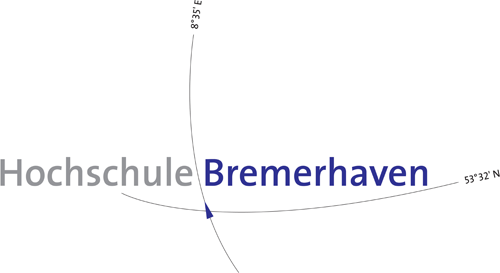
\includegraphics[scale=0.4]{images/hs-logo.png}
	\end{figure}
	\vspace*{1.0in}
	\hspace*{-1.3in}\colorbox{TitleBox}{
		\centering
		\parbox[t]{1.0\paperwidth}{
			\vspace*{0.7in}
			
			\centering
			\Large\textbf{\sTitle} \\
			
			\vspace*{0.7cm}
			\large{\sCaption}
			
			\vspace*{0.7in}
			
		}
	}
	\vfill{\centering \large
		\hfill \sName \\
		\hfill \sMtrNr \\
		\hfill \sUni \\
		\hfill \sDepartment \hspace{2mm}- \sFaculty \\
	}
\end{titlepage}

\newpage

\thispagestyle{empty}
\vspace*{2.0in}
\parbox[t]{1.0\linewidth}{ 
	\vspace*{0.7cm}
	
	\centering
	\Large\textbf{\sTitle} \\
	\vspace*{0.7cm}
	\large{\TitleDescription}
	

}
\vfill{
	\sArtofExam eingereicht im Rahmen des \sModul \\
	im Studiengang \sFaculty \hfill \\
	im \sDepartment\hfill \\
	der \sUni \hfill \\
	\\
	Betreuender Prüfer: \sFirstTutor \hfill \\
	Zweitgutachter: \sSecondTutor \hfill \\
	\\
	Abgabe am \sSubmissiondate

	\begin{titlepage}	
	\begin{figure}[h]
		\flushright
    	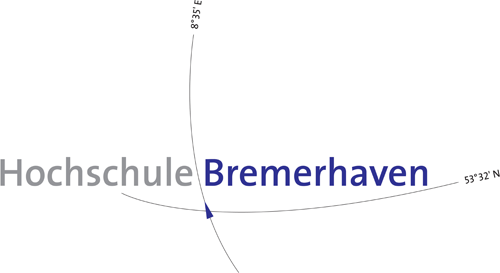
\includegraphics[scale=0.4]{images/hs-logo.png}
	\end{figure}
	\vspace*{1.0in}
	\hspace*{-1.3in}\colorbox{TitleBox}{
		\centering
		\parbox[t]{1.0\paperwidth}{
			\vspace*{0.7in}
			
			\centering
			\Large\textbf{\sTitle} \\
			
			\vspace*{0.7cm}
			\large{\sCaption}
			
			\vspace*{0.7in}
			
		}
	}
	\vfill{\centering \large
		\hfill \sName \\
		\hfill \sMtrNr \\
		\hfill \sUni \\
		\hfill \sDepartment \hspace{2mm}- \sFaculty \\
	}
\end{titlepage}

\newpage

\thispagestyle{empty}
\vspace*{2.0in}
\parbox[t]{1.0\linewidth}{ 
	\vspace*{0.7cm}
	
	\centering
	\Large\textbf{\sTitle} \\
	\vspace*{0.7cm}
	\large{\TitleDescription}
	

}
\vfill{
	\sArtofExam eingereicht im Rahmen des \sModul \\
	im Studiengang \sFaculty \hfill \\
	im \sDepartment\hfill \\
	der \sUni \hfill \\
	\\
	Betreuender Prüfer: \sFirstTutor \hfill \\
	Zweitgutachter: \sSecondTutor \hfill \\
	\\
	Abgabe am \sSubmissiondate

	\newpage

%----------------------------------------------------------------------------------------
%	ABSTRACT
%----------------------------------------------------------------------------------------
	\addchap*{Abstract}
\thispagestyle{empty}

 \addsec*{Thema}
 \sTitle

 \addsec*{Stichworte}
 Hier Stichworte, Stichworte, Stichworte, Stichworte

\addsec*{Kurzzusammenfassung}
In diesem Dokument findet ihr eine Erklärung und Vorlage zu LaTeX. Da auf English: \url{https://github.com/VoLuong/Begin-Latex-in-minutes}.

	\newpage
	
%----------------------------------------------------------------------------------------
%	Explanation
%----------------------------------------------------------------------------------------
	\addchap*{Erklärung}
\thispagestyle{empty}

Hiermit erkläre ich gegenüber dem \sDepartment der \sUni,

\begin{itemize}
	\item dass die vorliegende Arbeit mit dem Thema "\sTitle : \sCaption" \ von mir
	persönlich, selbstständig und ausschließlich unter Zuhilfenahme der im Literaturverzeichnis genannten Werke und
	Dokumente angefertigt wurde und dass keine fremde Hilfe in Anspruch genommen haben.
	\item dass die Arbeit weder vollständig noch in Teilen von mir selbst noch von anderen als Leistungsnachweis andernorts eingereicht wurde.
	\item dass ich wörtlich oder sinngemäß übernommene Textteile aus Schriften anderer Autoren als Zitate
	gekennzeichnet und die jeweilige Quelle im Literaturverzeichnis am Ende der Arbeit aufgeführt habe.
	\item dass ich alle Zeichnungen, Skizzen, Grafiken, Illustrationen, Fotografien und sonstige bildlichen	Darstellungen jeder Art sowie Ton - und Datenträger anderer Urheber als Übernahmen gekennzeichnet und die jeweilige Quelle im Literaturverzeichnis am Ende der Arbeit aufgeführt habe.
\end{itemize}

Mir ist bekannt, dass gegebenenfalls eine Überprüfung der hier vorgelegten Arbeit mittels einer
Antiplagiat-Software vorgenommen wird. Dafür stelle ich auf Nachfrage eine digitale, durchsuchbare Kopie dieser Arbeit zur Verfügung.

Mir ist bekannt, dass die Einreichung einer Arbeit unter Verwendung von Material, welches nicht als das geistige Eigentum anderer Personen gekennzeichnet wurde, ernsthafte Konsequenzen nach sich zieht.

\vspace {0.5cm}

Bremerhaven, \today \qquad

\begin{minipage}[hbt]{3in}
\vspace {0.5cm}
	
\includegraphics[scale=0.15]{images/signatur.png} \\
	\sName \ (\sMtrNr)
\end{minipage}
	\newpage
	
%----------------------------------------------------------------------------------------
%	TABLE OF CONTENTS
%----------------------------------------------------------------------------------------
	\begin{spacing}{1.0}
 		\tableofcontents
 		\newpage 
	\end{spacing}
	\newpage

%----------------------------------------------------------------------------------------
%	GLOSSAR
%----------------------------------------------------------------------------------------
	\pagenumbering{Roman} 
	\setcounter{page}{1}
	\addchap{Glossar}
\thispagestyle{empty}
\begin{acronym}
	\acro{AD}{Active Directory}\\
	Name des Verzeichnisdienstes von Microsoft Windows Server. Ab der Version 2008 umbenannt in \textbf{Active Directory Domain Services} (ADDS)
	\acro{AES}{Advanced Encryption Standard}
	\acro{AIS}{Application Interface Specification}
	\acro{ARP}{Address Resolution Protocol}\\
	Ein Netzwerkprotokoll welches zu einer IP-Adresse die physikalische Adresse zuordnet und ggf. in einer Tabelle hinterlegt.
\end{acronym}

	\newpage

%----------------------------------------------------------------------------------------
%	CHAPTERs
%----------------------------------------------------------------------------------------
%	\setcounter{page}{1}
%	\pagenumbering{arabic}
	\mainmatter  % isntead of the 2 lines before
	\chapter{Einleitung}
Willkommen zur Einführung in die Vorlage für eure schriftlichen Leistungsnachweise bzw. Bachelor- oder Masterbschlussarbeiten. Wir werden gemeinsam den Inhalt der Latex Vorlage durchgehen und dabei die Vorteile und Möglichkeiten von Latex ergründen. Beginnen wir mit der Dateistruktur dieser Vorlage.

\begin{itemize}
	\item Vorlage/
		\begin{itemize}
			\item bib/ - Unter diesem Ordner findet ihr die Bibtex Datei welche ihr mit Programmen wie readcube oder Jabref bearbeiten könnt. \url{http://www.jabref.org/}. Außerdem interessant für alle \url{https://www.mendeley.com/} und \url{http://www.citeulike.org/}
			\item chapter/ - In diesem Ordner werden sämtliche Latex .tex Dateien abgelegt in denen ihr euren Text verfasst. Ein Tipp: verteilt die Kapitel und Sektionen auf verschiedene Dateien. Dies ermöglicht ein paralleles Arbeiten und erleichtert die Arbeit an längeren Texten.
			\item images/ - Wie der Name schon sagt, ist dies der Ordner für Bilder aller Art. Benutzt dabei am besten .png, .svg oder .pdf da diese Dateiformate verlustfrei beim skalieren der Größe sind.
			\item lib/ - Hier sind sämtliche Dateien abgelegt mit denen das Aussehen des Dokumentes verändert werden kann. 
		\end{itemize}
\end{itemize}

Wenn ihr \textbf{komplette Neulinge} in LaTeX seid schaut gleichzeitig hier vorbei: \\\url{http://latex.tugraz.at/latex/tutorial}\\
\url{https://github.com/VoLuong/Begin-Latex-in-minutes}\\
http://texwelt.de/wissen/\\
Für alle die im Browser kollaborativ arbeiten möchten empfiehlt es sich \url{www.overleaf.com} zu nutzen. Wenn man lieber auf seinem PC arbeiten möchte, ist unter Windows die Tex-Umgebung \url{miktex.org} zu installieren. Auf dem Betriebssystem Linux muss in einem Terminal folgender Befehl eingegeben werden: "'sudo apt-get install texlive-full"'. Damit werden sämtliche Pakete und Sprachen heruntergeladen. Auf beiden Betriebssystemen bietet es sich an den Tex-Editor \emph{TexStudio} zu nutzen. Es gibt jedoch noch andere: \url{https://en.wikipedia.org/wiki/Comparison_of_TeX_editors}.

Bei weiteren Fragen oder Problemem zur Installation von Tex hier ein Link:\\
\url{http://texwelt.de/wissen/fragen/11038/wie-installiere-ich-latex}

\section{Wie beginnt man?}

Ein jedes Dokument beginnt man damit, die Metadaten zu bearbeiten und das Titelblatt einzustellen. In der Index TeX Datei "'Index.tex"' findet man dazu unter dem Abschnitt TITLE-Page zwei \textbf{input} Befehle die zu den Seiten \textbf{titlepage\_alone} und \textbf{titlepage\_group} verweisen. Wie die Namen schon aussagen ist jeder der Seiten für eine Sache optimiert. Bei einer Gruppe ab drei Personen wird empfohlen die Gruppenversion zu nehmen. Die Auswahl ist natürlich jedem selbst überlassen.\\

Weiter geht es zu den Metadaten in der Tex-Datei \textbf{person-configuration} in dem Ordner \emph{lib/}. Dort sollten sämtliche Informationen hinter den Befehlen angepasst werden. Die ersten Veränderungen können dann bereits auf dem Deckblatt verzeichnet werden.


\section{Aufbau der Index Datei}

Die Index-Datei beinhaltet die Struktur des Dokumentes. Sie ist eingeteilt in die Abschnitte:
\begin{itemize}
	\item Preamble: Hier werden die Einstellungen für das 'scrbook' übergeben. Wenn ihr eine anderes Aussehen möchtet, probiert stattdessen 'article'
	\item Einstellungen: Hier werden die Einstellungen zu Packages, Nutzerinformationen und Aussehen der Seiten geladen
	\item Bereich des Dokumentes: In diesem Segment wird die Abfolge des Dokumentes festgelegt. 
	\begin{itemize}
		\item Title-Page: Es stehen zwei Arten von Deckblättern zur Verfügung. Für Einzel- und Gruppenarbeiten.
		\item ABSTRACT: Auf dieser Seite muss das Thema des Leistungsnachweises kurz und bündig beschrieben werden.
		\item Explanation: In der Erklärung weist man darauf hin, dass kein Plagiat angefertigt wurde. Vergesst nicht zu unterschreiben bevor ihr abgebt.
		\item TABLE OF CONTENTS: Unter diesem Abschnitt wird festgelegt in welcher Reihenfolge die Gliederungen geordnet werden. Dabei ist interessant, dass mit dem Befehl \emph{pagenumbering} die Nummerierung auf "'Roman"' gesetzt wird und mit \emph{setcounter} die Zählung bei 1 zurückgesetzt wird.
		\item GLOSSAR: Hier sollten Fremdbegriffe welche im Dokument vorkommen mit kurzer Definition erklärt werden, sodass die Abkürzungen im Dokument benutzt werden kann.
		\item CHAPTERS: Hier bindet ihr eure Kapitel und Abschnitte ein.
		\item BIBLIOGRAPHY: Literaturverzeichnis wird am besten mit Jabref gepflegt
		\item APPENDIX: Wenn ihr einen Anhang benötigt für größere Bilder oder Diagramme, ist hier der richtige Ort dafür.
	\end{itemize}
\end{itemize}


\section{Pakete und CTAN}

Im Umgang mit LaTex werden sie sehr schnell auf das Problem stoßen das sie etwas tun möchten was von den in diesem Template vorhandenen Paketen nicht unterstützt wird. Um die Funktionalität hinzuzufügen suchen sie über eine Suchplattform (DuckDuckGo, Google etc.) ihrer Wahl nach dem richtigen \LaTeX Paket. In der Datei "'/lib/packages.tex"' sollten sie das Paket mittels des Befehls \verb|\usepackage{package}| einbinden. Sie können diesen Befehl überall im Dokument platzieren, der Übersicht halber sollte dies jedoch in der "'/lib/packages.tex"' geschehen. Nachdem das Paket eingebunden ist werden sie beim nächsten Compilieren ihres Dokumentes gefragt ob das Paket heruntergeladen werden soll. Bei der Installation haben sie bereits ein Repository einer unabhängigen Universität oder Hochschule ausgewählt. Jedes Paket hat ein Dokumentation, welche auf der Webseite \url{https://ctan.org} zu finden ist. Es empfiehlt sich stets die Dokumentation zu lesen, da diese meistens jede aufkommende Frage beantwortet. 
	\chapter{Drucken der Arbeit}
\label{chap:Drucken}



\section{Drucken}

\subsection{Drucker und Papier}

Die Arbeit sollte in der Endfassung unbedingt auf einem
qualitativ hochwertigen Laserdrucker ausgedruckt werden, Ausdrucke
mit Tintenstahldruckern sind \emph{nicht} ausreichend. Auch das
verwendete Papier sollte von guter Qualität (holzfrei) und
üblicher Stärke (mind.\ $80\; {\mathrm g} / {\mathrm m}^2$) sein.
Falls \emph{farbige} Seiten notwendig sind, sollte man diese einzeln%
\footnote{Tip: Mit \emph{Adobe Acrobat} lassen sich sehr einfach einzelne Seiten
des Dokuments für den Farbdruck auswählen und zusammenstellen.}
auf einem Farb-Laserdrucker ausdrucken und dem Dokument beifügen.

Übrigens sollten \emph{alle} abzugebenden Exemplare {\bf
gedruckt} (und nicht kopiert) werden! Die Kosten für den Druck
sind heute nicht höher als die für Kopien, der
Qualitätsunterschied ist jedoch --  bei Bildern und Grafiken
-- meist deutlich.


\subsection{Druckgröße}

Zunächst sollte man sicherstellen, dass die in der fertigen PDF-Datei eingestellte
Papiergröße tatsächlich \textbf{A4} ist! Das geht z.B.\ mit \emph{Adobe Acrobat}
oder \emph{SumatraPDF}
über \texttt{File} $\rightarrow$ \texttt{Properties},
wo die Papiergröße des Dokuments angezeigt wird:
\begin{center}
\textbf{Richtig:} A4 = $8{,}27 \times 11{,}69$ in bzw.\ $21{,}0 \times 29{,}7$ cm.
\end{center}

Ein häufiger und leicht zu übersehender Fehler beim Ausdrucken von
PDF-Dokumenten wird durch die versehentliche Einstellung der
Option "`Fit to page"' im Druckmenü verursacht, wobei die Seiten
meist zu klein ausgedruckt werden. Überprüfen Sie daher die Größe
des Ausdrucks anhand der eingestellten Zeilenlänge oder mithilfe
einer Messgrafik, wie am Ende dieses Dokuments gezeigt.
Sicherheitshalber sollte man diese Messgrafik bis zur
Fertigstellung der Arbeit beizubehalten und die entsprechende
Seite erst ganz am Schluss zu entfernen.
Wenn, wie häufig der Fall, einzelne Seiten getrennt in Farbe gedruckt 
werden, so sollten natürlich auch diese genau auf die Einhaltung der Druckgröße 
kontrolliert werden!




\section{Binden}

Die Endfassung der Leistungsnachweises ist je nach Vorgaben des Studiengangs, meist eine einfache Bindung einzureichen. Diese kann man im ASTA-Büro oder in Copyshops drucken bzw. binden lassen.

Falls man im Falle einer Bachelorarbeit oder Masterarbeit die Arbeit bei einem
professionellen Buchbinder durchführen lässt, sollte man auch auf
die Prägung am Buchrücken achten, die kaum zusätzliche Kosten
verursacht. Üblich ist dabei die Angabe des Familiennamens des
Autors und des Titels der Arbeit. Ist der Titel der Arbeit zu
lang, muss man notfalls eine gekürzte  Version angeben, wie z.B.:
%
\begin{center}
\setlength{\fboxsep}{3mm}
\fbox{
\textsc{Schlaumeier}
\textperiodcentered\ \textsc{Parz.\ Lösungen zur allg.\ Problematik}}
\end{center}
%



\section{Elektronische Datenträger (CD-R, DVD)}
Speziell bei Arbeiten im Bereich der Informationstechnik (
nicht nur dort) fallen fast immer Informationen an, wie Programme,
Daten, Grafiken, Kopien von Internetseiten usw., die für eine
spätere Verwendung elektronisch verfügbar sein sollten.
Vernünftigerweise wird man diese Daten während der Arbeit bereits
gezielt sammeln und der fertigen Arbeit auf einer CD-ROM oder DVD
beilegen. Es ist außerdem sinnvoll -- schon allein aus Gründen der
elektronischen Archivierbarkeit -- die eigene Arbeit selbst als
PDF-Datei beizulegen.%
\footnote{Auch Bilder und Grafiken könnten in elektronischer Form nützlich
sein, die LaTeX- oder Word-Dateien sind hingegen überflüssig.}


Falls ein elektronischer Datenträger (CD-ROM oder DVD) beigelegt
wird, sollte man auf folgende Dinge achten:
%
\begin{enumerate}
\item Jedem abzugebenden Exemplar muss eine identische Kopie des
Datenträgers beiliegen. %
\item Verwenden Sie qualitativ hochwertige Rohlinge und überprüfen
Sie nach der Fertigstellung die tatsächlich gespeicherten Inhalte
des Datenträgers! %
\item Der Datenträger sollte in eine im hinteren Umschlag
eingeklebte Hülle eingefügt sein und sollte so zu entnehmen sein,
dass die Hülle dabei \emph{nicht} zerstört wird (die
meisten Buchbinder haben geeignete Hüllen parat). %
\item Der Datenträger muss so beschriftet sein, dass er der
Leistungsnachweis eindeutig zuzuordnen ist, am Besten durch ein
gedrucktes Label%
\footnote{Nicht beim lose abgegebenen Bibliotheksexemplar --
dieses erhält ein standardisiertes Label durch die Bibliothek.} %
oder sonst durch \emph{saubere}
Beschriftung mit
der Hand und einem feinen, wasserfesten Stift. %
\item Nützlich ist auch ein (grobes) Verzeichnis der Inhalte des
Datenträgers
\end{enumerate}

	\chapter{Strukturen in Latex}

In Latex werden Kapitel mit \verb+\chapter{}+ erstellt. Ein Abschnitt wird mit \verb+\section{}+ und einen Absatz mit \verb+\paragraph+ definiert. Sie können auch einen Unterabschnitt mit \verb+\subsection{}+ und einen Unterabsatz mit \verb+\subparagraph{}+ hinzufügen.\\

Es gibt ebenso noch die \verb|\\|, \verb|\\\\| sowie \verb|\newline| um einen Text um eine Zeile zu verrücken. \newline

Sie sollten Unterabschnitte stets nur bis zur zweiten Ebene unterteilen. Manchmal wird auch die dritte Ebene erlaubt. Dies ist vom Professor abhängig. Wenn es dennoch notwendig sein sollte, eine höhere Anzahl an Unterabschnitten hinzuzufügen, zum Beispiel bis in die 100te Ebene, hilft folgender Link dabei: \url{https://tex.stackexchange.com/questions/30997/more-section-headings}.\newline



Die Umgebung \verb|\begin{quote}\end{quote}| sollte genutzt werden um Zitate im Text einfließen zu lassen. Es können aber auch die Anführungszeichen \verb|"'Text"'| genutzt werden.

\begin{quote}
	Der Mensch ist immer noch der beste Computer.\\
	John F. Kennedy \cite{jfkey}
\end{quote}

	\chapter{Header und Footer}
%http://www.mychemistry.eu/2013/05/about-footnotes/
In Latex ist es möglich die Seiteneinstellung anzupassen. Unter anderem können die Kopfzeile und Fußzeile angepasst werden. Die Anpassungsmöglichkeiten beziehen sich auf die Breite und Höhe sowie Inhalt der Zeilen. Umgesetzt wird dies in der Praxis mit den Paketen \emph{fancyhdr} und \emph{titleps}. 

\begin{description}
	\item[fancyhdr:] Das Paket bietet umfangreiche Möglichkeiten, sowohl für die Erstellung von Kopf- und Fußzeilen als auch für die Steuerung ihrer Verwendung (z.B. in Zeiten, in denen LATEX automatisch den verwendeten Überschriften-Stil ändert).\\
	\url{https://ctan.org/pkg/fancyhdr}
	\item[titleps:] Das Paket bietet Seitenstile mit einem einfachen einstufigen Mechanismus, einschließlich Bestnoten, Zugriff auf Top-, First- und Botmarks in einem einzigen Header/Footer, Header/Footer für bestimmte Floats, mehrere Sätze von Marken (mit e-TEX) und mehr.
	Das Paket ist Teil der titleec-Distribution.\\
	\url{https://ctan.org/pkg/titleps}
\end{description}

Im ersten Beispiel wird die generelle Nutzung gezeigt von \emph{fancyhdr}. Das Ergebnis des LaTeX Quellcodes wird mit dem package \emph{pdfpages} eingebunden. Im zweiten Beispiel wird gezeigt wie in der Fußzeile die aktuelle Seitenzahl zur Gesamtanzahl der Seiten mit Hilfe des Paketes \emph{lastpage} angezeigt werden kann.
\newpage
\begin{lstlisting}[style=LaTeX]
\documentclass[12pt]{article}
\usepackage{titleps} % für die Seitenstile
\usepackage{fancyhdr} % für die Kopfzeile und Fußzeile
\usepackage{graphicx} % für das example-iamge-a
\usepackage{lipsum} % für dummy text

\pagestyle{myheadings}
\pagestyle{fancy}
\fancyhf{}

\setlength{\headheight}{30pt} % Höhe der Kopfzeile

\renewcommand{\headrulewidth}{4pt} % Dicke der Kopzeile
\renewcommand{\footrulewidth}{2pt} % Dicke der Fußzeile

\fancyhead[L]{\includegraphics[width=1cm]{example-image-a}}
\fancyhead[C]{} % Option C bedeutet Center wie (L)eft
\fancyhead[R]{\rightmark}
\fancyfoot[L]{ABC}
\fancyfoot[C]{\textcopyright xyz}
\fancyfoot[R]{\thepage}


\begin{document}

\section{First section}
\subsection{One}
\lipsum[1-3]
\subsection{Two}
\lipsum[4-6]

\end{document}
\end{lstlisting}

% Package pdfpages https://www.namsu.de/Extra/pakete/Pdfpages.html
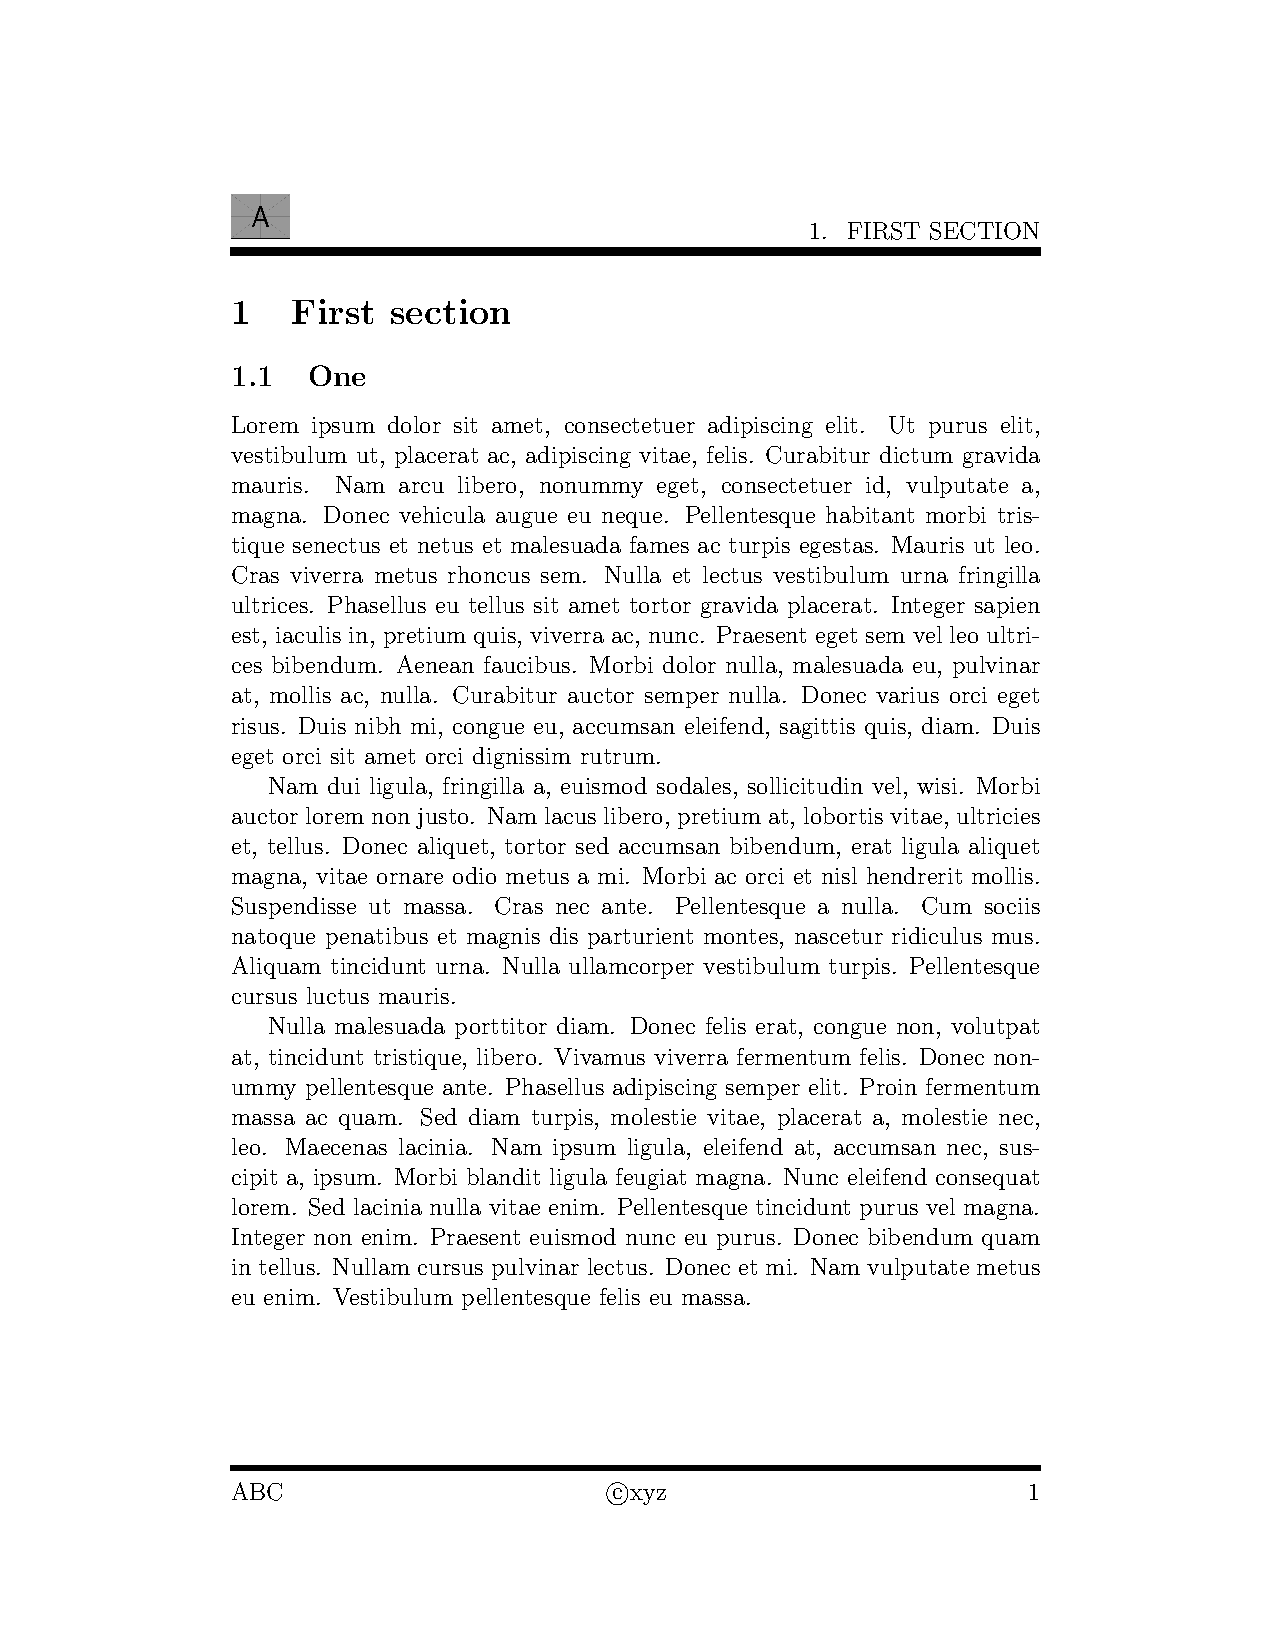
\includepdf[pages=-]{examples/header-footer} 

\begin{lstlisting}[style=LaTeX]
\documentclass[12pt]{article}
\usepackage{lastpage}
\usepackage{fancyhdr}
\usepackage{graphicx}
\usepackage{lipsum} % for dummy text
\pagestyle{myheadings}
\pagestyle{fancy}
\fancyhf{}
\setlength{\headheight}{30pt}
\renewcommand{\headrulewidth}{1pt}
\renewcommand{\footrulewidth}{2pt}
\lhead{\includegraphics[width=1cm]{example-image-a}}
\rhead{}
\lfoot{ABC}
\rfoot{\thepage/\pageref{LastPage}}
\begin{document}
\subsection{One}
\lipsum[1-3]
\subsection{Two}
\lipsum[4-6]
\end{document}
\end{lstlisting}

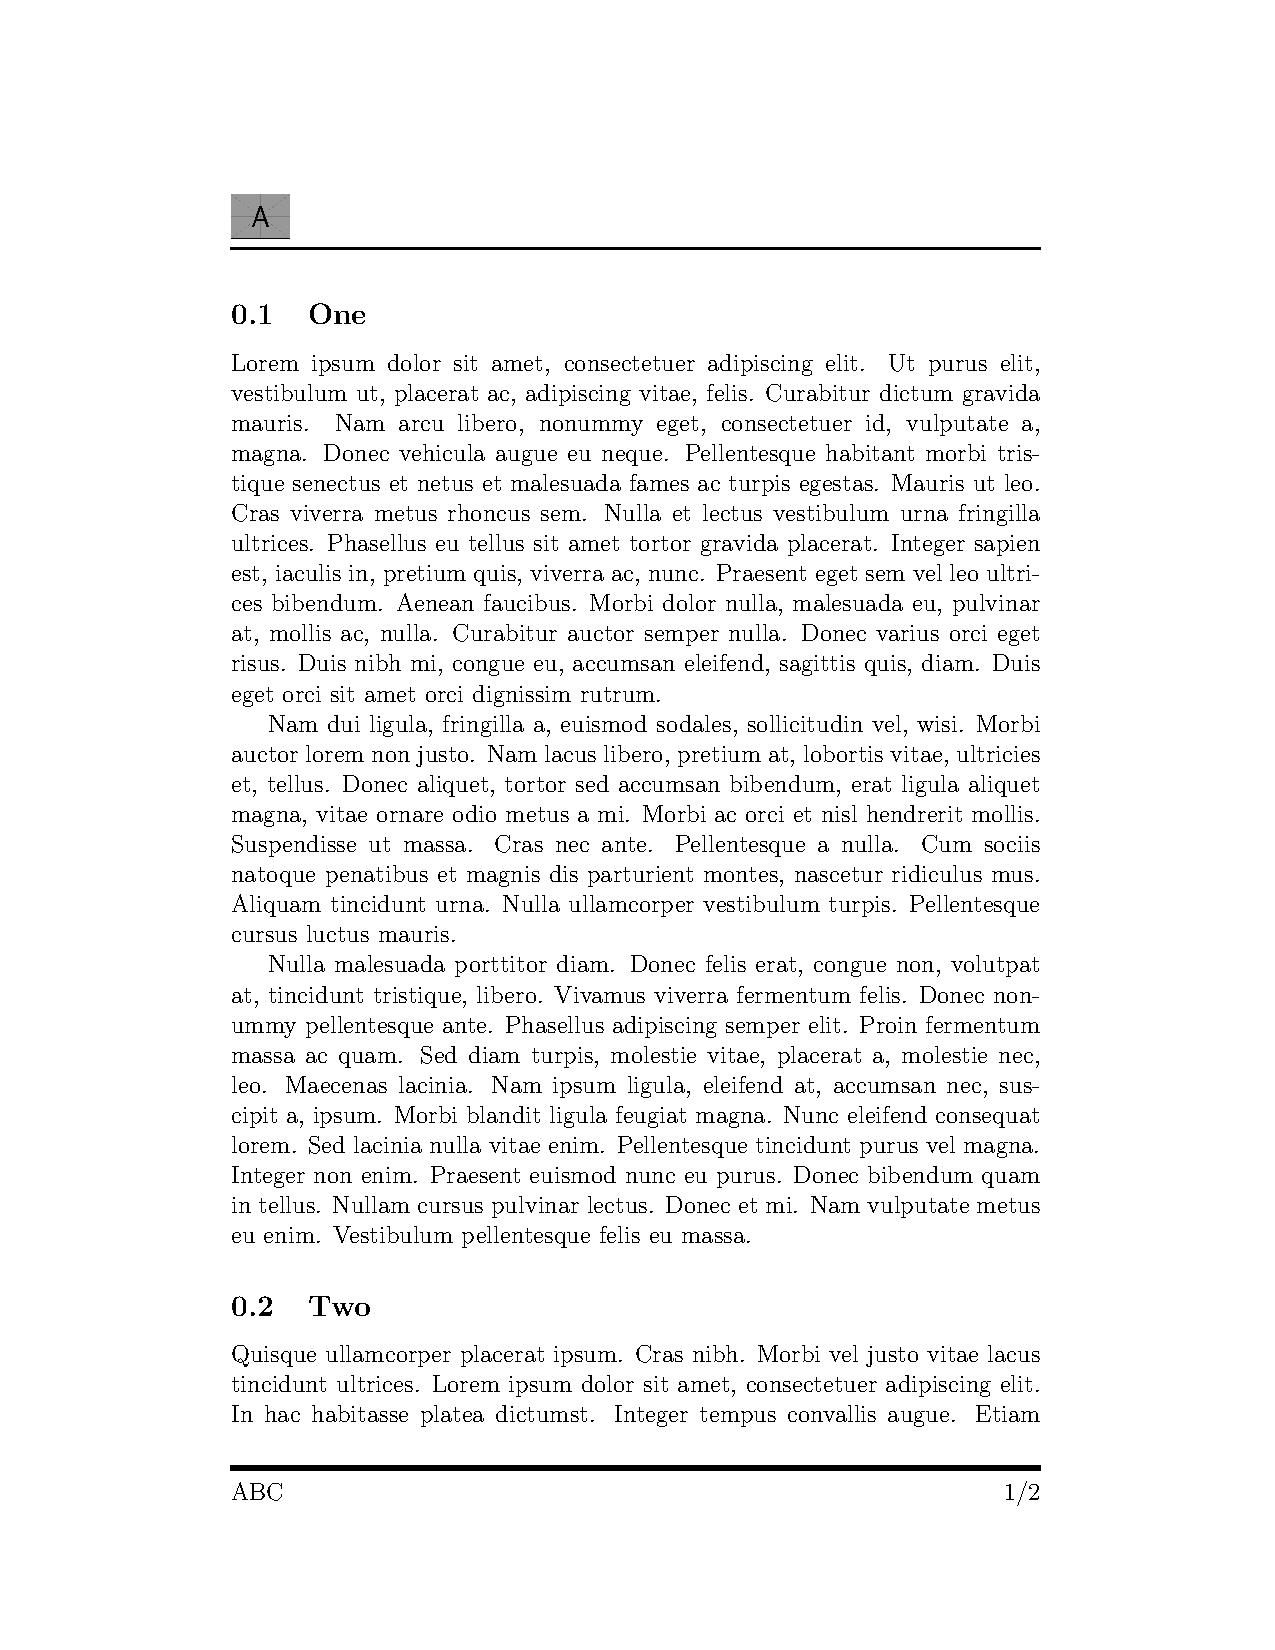
\includepdf[pages=-]{examples/header-footer-lastpage} 

	\chapter{Tabellen}

Tabellen werden in der zugehörigen Umgebung geschrieben \verb|\begin{table}\end{table}|

% Wie sehen Tabellen aus wie funktionieren sie
% Was hat es mit ResizeBox auf sich
% Was ist Tabular
% Eine Zeile mit anderer Ausrichtung statt die Ausrichtung der Spalte
% LongTables erklären
% Bestimmte Seiten als Querformat
	
% Einfärben?


	\chapter{Listen}

Listen in Listen

Listen mit weniger Platz zwischen den Zeilen
	\chapter{Bilder}

Um Bilder in \LaTeX{} einzufügen wird der Befehl \verb|\includegraphics[Option]{Pfad/Dateiname}| genutzt. Näheres zu dem Befehl hier: \url{http://www.golatex.de/wiki/%5Cincludegraphics}

Diese Optionen sind nur verfügbar, wenn zuvor das graphicx-Paket eingebunden wurde. Andere Pakete wie graphics unterstützen nicht alle Optionen.	
\begin{itemize}
\item angle - Bestimmt den Drehwinkel um einen Referenzpunkt für die Grafik. Positive Werte drehen die Grafik gegen den Uhrzeigersinn, negative mit ihm.
\item draft - Ist draft gesetzt, wird nur ein Platzhalter der Grafik angezeigt. Beschleunigt den Übersetzungsvorgang des Dokuments erheblich. Oftmals kann draft auch in den Dokumentoptionen angegeben werden.
\item scale - Skaliert die Grafik anhand eines Skalierungsfaktors.
\item height - Skaliert die Grafik auf die angegebene Höhe. Die Angabe der Größe muss in einer LaTeX-spezifischen Einheit erfolgen.
\item width - Skaliert die Grafik auf die angegebene Breite. Die Angabe der Größe muss in einer LaTeX-spezifischen Einheit erfolgen.
\end{itemize}	
% Wie fügt man Bilder ein
	% Wie muss Caption gemacht werden bzw. keine Caption
% Wie bekommt man Bilder nebeneinander
% Wie bekommt man Bilder umflossen vom Text

\begin{figure}[ht]
	\centering
	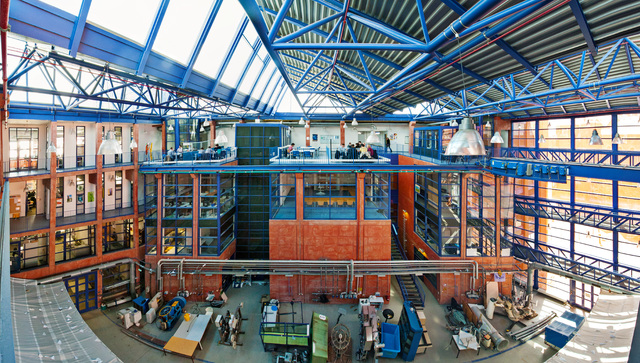
\includegraphics{images/Haus_Z.jpeg}
	\caption{Innenraum von Haus Z \autocite{hauszpic}}
	\label{fig1}
\end{figure}

\verb|\includegraphics| muss nicht zwingend in einer figure-Gleitumgebung verwendet werden, ratsam ist es aber schon, da sonst keine Bildunterschriften bzw. Bezeichner gesetzt werden können. Die Bildunterschriften haben dabei immer unter dem Bild zu sein mit einem \verb|\autocite{text}| auf den Ursprungsort des Bildes. Der Befehl \verb|\autocite{text}| greift auf die \emph{.bib} Datei über den Bibtexkey zu. Weitere Informationen zur figure-Gleitumgebung finden sie hier: \url{https://en.wikibooks.org/wiki/LaTeX/Floats,_Figures_and_Captions}\newline

Auch Bilder können nebenbeinander platziert werden. Dies kann auf sehr verschiedene Weise erreicht werden: \url{http://texwelt.de/wissen/fragen/18877/zwei-bilder-nebeneinander-jeweils-mit-bildunterschrift-und-label} 

Als Beispiel wird in diesem Dokument das Paket \emph{floatrow} genutzt.
\begin{quote}
	"'Das Paket floatrow bietet zwei Features, die für die Umsetzung der Anforderung verwendet werden können.
	
	Zum einen kann man mit \verb|\ffigbox| eine Abbildung zusammen mit ihrer Bildunterschrift in genau der Breite setzen, die durch die Abbildung vorgegeben wird. Das funktioniert auch dann noch, wenn die Bildunterschrift mehrzeilig wird. Dazu ist als optionales erstes Argument \verb|\FBwidth| anzugeben. Als zweites Argument wird \verb|\caption[…]{…}| zusammen mit einem ggf. zu setzenden \verb|\label{…}| angegeben. Das dritte Argument ist die Abbildung.
	
	Desweiteren bietet das Paket die Möglichkeit, durch \verb|\ffigbox| angegebene Abbildungen innerhalb einer floatrow-Umgebung in Spalten nebeneinander anzuordnen. Für zwei Abbildungen nebeneinander muss man die beiden durch \verb|\ffigbox| definierten Abbildungen also nur zusätzlich in eine floatrow-Umgebung packen."'\autocite{floatrow}
\end{quote}
\begin{figure}[h]
	\centering
	\begin{floatrow}
		\ffigbox[\FBwidth]{%
			\caption{Linke Abbildung}\label{fig:left}
		}{%
			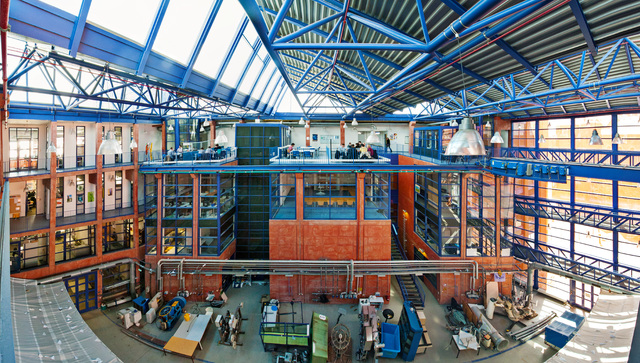
\includegraphics[scale=1]{images/Haus_Z.jpeg}
		}%
		\ffigbox[\FBwidth]{%
			\caption{Abbildung rechts neben der linken Abbildung}\label{fig:right}
		}{%
			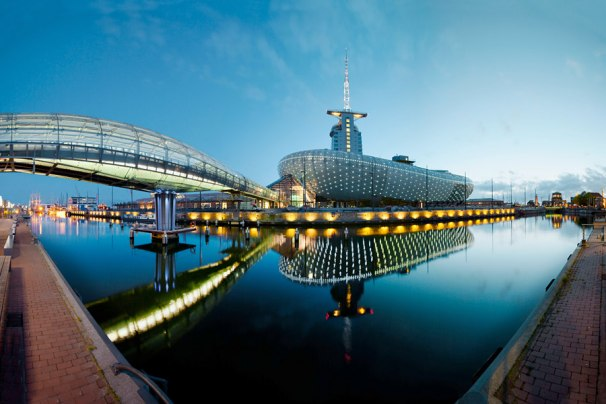
\includegraphics[scale=.3]{images/Klimahaus.jpeg}
		}%
	\end{floatrow}
\end{figure}

Um Bilder in einem Text zu platzieren sodass das Bild davon umschlossen wird, muss eine \verb|\wrapfigure| Umbegung genutzt werden.\\

\verb|\begin{wrapfigure}[Zeilen]{Position}[Ueberhang]{Breite}|\\
Um das Margin als den weißen Rand um das Bild zu reduzieren wird der Befehl \verb|\columnsep| des Paketes genutzt. Durch den Befehl \verb|\lipsum| erzeugt man Lorem Ipsum Text.\\

\lipsum[1-1]
\begingroup
\setlength{\columnsep}{-30pt} % verändert die Größe des Margin nach links und rechts
\setlength{\intextsep}{1pt}  %verändert die Größe des Margin nach oben und unten
\begin{wrapfigure}{R}{.6\textwidth}
	\begin{center}
		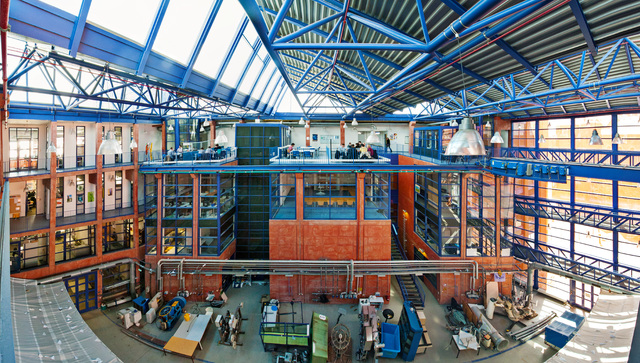
\includegraphics[width=0.6\textwidth]{images/Haus_Z.jpeg}
	\end{center}
	\caption{Rechtsbündig im Text \autocite{hauszpic}}\label{fig:classrr}
\end{wrapfigure}
%\lipsum[1-1]
Dies asdhkajsdhak shaudhasi dhasidh aipudh aipsudhai sdh aipdh aipsdhapi dugh aipdh aipdh aipsudg asipd gauidg aipdgaipdg apid gaipg aif gsipf as pifg wizf a wui fais fis ufpsiudfsi df sipduf siu fsid uf si f spi fgsiufgsiufgsidufgsdidufgsipdufsiufbsiufsidufsidufhsiufhsidofhisdouisufhsidu  sidufh sdiufzsdi ufzsdiüufz sdiuü fzsdz fdsiufz dsiu fzsdiufz sdiu fzsduifsudi zfsduifz sud9f zsüdu füdsif asdjaköjsdnökajsdnökajsdhökajsdbnköajjs a shdpahs dpiau sdh ipau sdhpia hsdiüoau hd piausdh piausdg piagdipasudghipaushd piausdhpiaus de.
%Man benötigt bei \endgroup eine Leere Zeile zwischen Text und dem Befehl oder man nutzt \par
\par
\endgroup





	\chapter[Mathem.\ Formeln etc.]{Mathematische Formeln, Gleichungen und Algorithmen}
\label{chap:Mathematik}

% Formelverzeichniss

Das Formatieren von mathematischen Elementen gehört sicher zu den
Stär\-ken von LaTeX. Man unterscheidet zwischen mathematischen Elementen
im Fließtext und freistehenden Gleichungen, die in der Regel
fortlaufend nummeriert werden. Analog zu Abbildungen und Tabellen sind dadurch
Querverweise zu Gleichungen leicht zu realisieren. Zum besseren Verständnis schaut euch neben dieser PDF auch den Quelltext in der Datei \emph{mathematik.tex} an.


\section{Mathematische Elemente im Fließtext}

Mathematische Symbole, Ausdrücke, Gleichungen etc.\ werden im Fließtext durch paarweise \verb!$! \ldots \verb!$! markiert. Hier ein Beispiel:
%
\begin{quote}
Der Nah-Unendlichkeitspunkt liegt bei
$\bar{a} = f' \cdot \bigl( \frac{f'}{K \cdot u_{\max}} + 1 \bigr)$,
sodass bei einem auf $\infty$ eingestellten Objektiv von der Entfernung
$\bar{a}$ an alles scharf ist. Fokussiert man das
Objektiv auf die Entfernung $\bar{a}$ (dass heißt, $a_0 = \bar{a}$), dann wird
im Bereich $[\frac{\bar{a}}{2}, \infty]$ alles scharf.
\end{quote}
%
Dabei sollte man unbedingt darauf achten, dass die Höhe der einzelnen Elemente im Text nicht zu groß wird. 

\paragraph{Häufiger Fehler:} 
Im Fließtext wird bei einfachen Variablen oft auf die Verwendung der richtigen, mathematischen Zeichen vergessen, wie etwa in 
"`X-Achse"' anstelle von "`$X$-Achse"' (\verb!$X$-Achse!).



\section{Freigestellte Ausdrücke}

Freigestellte mathematische Ausdrücke können in LaTeX im einfachsten Fall durch paarweise \verb!$$! \ldots \verb!$$! erzeugt werden. Das Ergebnis wird zentriert, erhält jedoch keine Numerierung. So ist z.B.\ $$ y = 4 x^2 $$ das Ergebnis von \verb!$$ y = 4 x^2 $$!.

\subsection{Einfache Gleichungen} 

Meistens verwendet man in solchen Fällen jedoch die \texttt{equation}-Umgebung zur Herstellung numerierter Gleichungen, auf die man im Text jederzeit verweisen kann. Zum Beispiel erzeugt
%

\begin{equation}
  f(k) = \frac{1}{N} \sum_{i=0}^{k-1} i^2 . 
  \label{eq:MyFirstEquation}
\end{equation}

%
die Gleichung
%
\begin{equation}
  f(k) = \frac{1}{N} \sum_{i=0}^{k-1} i^2 . 
\label{eq:MyFirstEquation}
\end{equation}
%
Mit \verb!\ref{eq:MyFirstEquation}! erhält man wie üblich die Nummer (\ref{eq:MyFirstEquation}) dieser Gleichung (siehe dazu auch Abschn.\ \ref{sec:VerweiseAufGleichungen}). 
Dieselbe Gleichung \emph{ohne} Numerierung kann man übrigens mit der \texttt{equation*}-Umgebung erzeugen.



\begin{center}
\setlength{\fboxrule}{0.2mm}
\setlength{\fboxsep}{2mm}
\fbox{%
\begin{minipage}{0.9\textwidth}
Man beachte, dass \textbf{Gleichungen} inhaltlich ein \textbf{Teil des Texts} sind und daher neben der sprachliche \textbf{Überleitung} auch die \textbf{Punktuation} (wie in Gl.\ \ref{eq:MyFirstEquation} gezeigt) beachtet werden muss. Bei Unsicherheiten sollte man sich passende Beispiele in einem guten Mathematik\-buch ansehen.
\end{minipage}}
\end{center}
%
Für Interessierte findet sich mehr zum Thema Mathematik und Prosa in \cite{Mermin89} und \cite{Higham98}.

\subsection{Mehrzeilige Gleichungen}

Für mehrzeilige Gleichungen bietet LaTeX die 
\verb!eqnarray!-Umgebung, die allerdings etwas eigenwillige Zwischenräume erzeugt.
Es empfiehlt sich, dafür gleich auf die erweiterten Möglichkeiten des \texttt{amsmath}-Pakets%
\footnote{American Mathematical Society (AMS). \texttt{amsmath} ist Teil der LaTeX Standardinstallation und wird von \texttt{hgb.sty} bereits importiert.}
\cite{amsldoc02} zurückzugreifen.
Hier ein Beispiel mit zwei am $=$ Zeichen ausgerichteten Gleichungen,
%
\begin{align}
f\_1 (x,y) &= \frac{1}{1-x} + y , \label{eq:f1} \\
f\_2 (x,y) &= \frac{1}{1+y} - x , \label{eq:f2}
\end{align}
%
erzeugt mit der \texttt{align}-Umgebung aus dem \texttt{amsmath}-Paket:
%

\begin{align}
  f\_1 (x,y) &= \frac{1}{1-x} + y , \label{eq:f11} \\
  f\_2 (x,y) &= \frac{1}{1+y} - x , \label{eq:f21}
\end{align}



\subsection{Fallunterscheidungen}

Mit der \texttt{cases}-Umgebung aus \texttt{amsmath} sind Fallunterscheidungen, unter anderem innerhalb von Funktionsdefinitionen, sehr einfach zu bewerkstelligen. Beispielsweise wurde die rekursive Definition
%
\begin{equation}
	f(i) =
	\begin{cases}
	  0             & \text{für $i = 0$},\\
	  f(i-1) + f(i) & \text{für $i > 0$}.
	\end{cases}
\end{equation}
mit folgenden Anweisungen erzeugt:
%

\begin{equation}
	f(i) =
	\begin{cases}
	  0             & \text{für $i = 0$},\\
	  f(i-1) + f(i) & \text{für $i > 0$}.
	\end{cases}
\end{equation}

%
Man beachte dabei die Verwendung des sehr praktischen \verb!\text{..}!-Makros, mit dem im Mathematik-Modus gewöhnlicher Text eingefügt werden kann, sowie wiederum die Punktuation innerhalb der Gleichung.

\subsection{Gleichungen mit Matrizen}

Auch hier bietet \texttt{amsmath} einige Vorteile gegenüber der Verwendung der LaTeX Standardkonstrukte. Dazu ein einfaches Beispiel für die Verwendung der \texttt{pmatrix}-Umgebung für Vektoren und Matrizen,
%
\begin{equation}
	\begin{pmatrix} x' \\ y' \end{pmatrix}
	= 
	\begin{pmatrix}
	  \cos \phi & -\sin \phi \\
	  \sin \phi & \phantom{-}\cos \phi
	\end{pmatrix} 
	\cdot
	\begin{pmatrix}	x \\ y \end{pmatrix} ,
\end{equation}
%
das mit den folgenden Anweisungen erzeugt wurde:
%

\begin{equation}
	\begin{pmatrix} 
			x' \\ 
			y' 
	\end{pmatrix}
	= 
	\begin{pmatrix}
		  \cos \phi & -\sin \phi \\
		  \sin \phi & \phantom{-}\cos \phi /+ \label{lin:phantom} +/
	\end{pmatrix} 
	\cdot
	\begin{pmatrix} 
			x \\ 
			y 
	\end{pmatrix} ,
\end{equation}

%
Ein nützliches Detail darin ist das TeX-Makro \verb!\phantom{..}! (in Zeile \ref{lin:phantom}), das sein Argument unsichtbar einfügt und hier als Platzhalter für das darüberliegende Minuszeichen verwendet wird. Alternativ zu \texttt{pmatrix} kann man mit der \texttt{bmatrix}-Umgebung Matrizen
und Vektoren mit eckigen Klammern erzeugen.
Zahlreiche weitere mathematische Konstrukte des \texttt{amsmath}-Pakets sind in \cite{amsldoc02} beschrieben.



\subsection{Verweise auf Gleichungen}
\label{sec:VerweiseAufGleichungen}

Beim Verweis auf nummerierte Formeln und Gleichungen genügt grundsätzlich die Angabe 
der entsprechenden Nummer in runden Klammern,
z.B.
\begin{center}
%"`\ldots\ wie aus (\ref{eq:f1}) abgeleitet werden kann \ldots"'
"`\ldots\ wie aus (\ref{eq:f1}) abgeleitet werden kann \ldots"'
\end{center}
Um Missverständnisse zu vermeiden, sollte man in Texten mit
nur wenigen mathematischen Elementen -- "`Gleichung \ref{eq:f1}"', "`Gl.~\ref{eq:f1}"' 
oder "`Gl.~(\ref{eq:f1})"' schreiben (natürlich konsistent). 
%\emph{Falsch} wäre hingegen "`Gleichung (\ref{eqn:zerstreuungskreis})"'.

\begin{center}
\setlength{\fboxrule}{0.2mm}
\setlength{\fboxsep}{2mm}
\fbox{%
\begin{minipage}{0.9\textwidth}
\textbf{Achtung:} Vorwärtsverweise auf (im Text weiter hinten liegende) Gleichungen sind \textbf{äußerst ungewöhnlich} 
und sollten vermieden werden! Glaubt man dennoch so etwas zu benötigen, dann wurde
meistens ein Fehler in der Anordnung gemacht.
\end{minipage}}
\end{center}


\section{Spezielle Symbole}

\subsection{Zahlenmengen}
Einige häufig verwendete Symbole sind leider im ursprünglichen
mathematischen Zeichensatz von LaTeX nicht enthalten, z.B. die
Symbole für die reellen und natürlichen Zahlen. 


\subsection{Operatoren}

In LaTeX\ sind Dutzende von mathematischen Operatoren für spezielle Anwendungen definiert. Am häufigsten werden natürlich die arithmetischen Operatoren $+$, $-$, $\cdot$ und $/$ benötigt. Ein dabei oft beobachteter Fehler (der wohl aus der Programmierpraxis resultiert) ist die Verwendung von $*$ für die einfache Multiplikation -- richtig ist $\cdot$ (\verb!\cdot!).%
\footnote{Das Zeichen $*$ wird üblicherweise für den Faltungsoperator verwendet.}
%
Für Angaben wie z.B. "`ein Feld mit $25 \times 70$ Metern"' (aber auch fast \emph{nur} dafür) verwendet man sinnvollerweise den $\times$ (\verb!\times!) Operator und \emph{nicht} einfach das Textzeichen~"`x"'!


\subsection{Variable (Symbole) mit mehreren Zeichen}
Vor allem bei der mathematischen Spezifikation von Algorithmen und Programmen
ist es häufig notwendig, Symbole (Variablennamen) mit mehr als einem Zeichen
zu verwenden, z.B.
%
$$Scalefactor\leftarrow Scalefactor^2 \cdot 1.5 \; ,$$
%
\textbf{fälschlicherweise} erzeugt durch 
\begin{quote}
	\verb!$Scalefactor \leftarrow Scalefactor^2! \verb!\cdot 1.5$!.
\end{quote}
Dabei interpretiert LaTeX allerdings die Zeichenkette "`Scalefactor"' als 11 einzelne,
aufeinanderfolgende Symbole $S$, $c$, $a$, $l$, $e$, \ldots und setzt dazwischen
entsprechende Abstände.
\textbf{Richtig} ist, diese Buchstaben mit
\verb!\mathit{..}! zu \emph{einem} Symbol zusammenzufassen.
Der Unterschied ist in diesem Fall deutlich sichtbar:
%
\begin{center}
\setlength{\tabcolsep}{4pt}
\begin{tabular}{llll}
\text{Falsch:}   & $Scalefactor^2$ & $\leftarrow$ & \verb!$Scalefactor^2$! \\
\text{Richtig:}  & $\mathit{Scalefactor}^2$ & $\leftarrow$ & \verb!$\mathit{Scalefactor}^2$!
\end{tabular}
\end{center}
%
Grundsätzlich sollte man aber derart lange Symbolnamen aber ohnehin vermeiden und stattdessen 
möglichst kurze (gängige) Symbole verwenden
(z.B.\ Brennweite $f = 50 \, \mathrm{mm}$ statt $\mathit{Brennweite} = 50 \, \mathrm{mm}$).

\subsection{Funktionen}

Während Symbole für Variablen traditionell (und in LaTeX\ automatisch) \emph{italic} gesetzt werden, verwendet man für die Namen von Funktionen und Operatoren üblicherweise
\emph{roman} als Schrifttyp, wie z.B. in
\begin{center}
\begin{tabular}{lcl}
	$\sin \theta = \sin(\theta + 2 \pi)$ & 
	$\leftarrow$ & \verb!$\sin \theta = \sin(\theta + 2 \pi)$! \\
	\end{tabular}
\end{center}
Das ist bei den bereits vordefinierten Standardfunktionen (wie
\verb!\sin!,
\verb!\cos!,
\verb!\tan!,
\verb!\log!,
\verb!\max!
) automatisch der Fall.
Diese Konvention sollte man auch bei selbstdefinierten Funktionen befolgen,
wie etwa in
\begin{center}
	\begin{tabular}{lcl}
	$\mathrm{Distance}(A,B) = |A-B|$ & $\leftarrow$ & \verb!$\mathrm{Distance}(A,B) = |A-B|$! \\
	\end{tabular}
\end{center}


\subsection{Maßeinheiten und Währungen}

Bei der Angabe von Maßeinheiten wird üblicherweise Normalschrift
(keine Italics) verwendet, z.B.:
\begin{quote}
Die Höchstgeschwindigkeit der \textit{Bell XS-1} beträgt 345~m/s
bei einem Startgewicht von 15~t. 
Der Prototyp kostete über 25.000.000 US\$, also ca.\ 19.200.000 \euro\ nach heutiger Umrechnung.
\end{quote}
Der Abstand zwischen der Zahl und der Maßeinheit ist dabei
gewollt.
Das \$-Zeichen erzeugt man mit \verb!\$! und
das Euro-Symbol (\euro) mit dem Makro \verb!\euro!.%
\footnote{Das \euro\ Zeichen ist nicht im ursprünglichen LaTeX-Zeichensatz enthalten
sondern wird mit dem \texttt{eurosym}-Paket erzeugt.}


\subsection{Kommas in Dezimalzahlen (Mathematik-Modus)}

LaTeX\ setzt im Mathematik-Modus (also innerhalb von \verb!$$! oder in Gleichungen) nach dem angloamerikanischen Stil in Dezimalzahlen grundsätzlich den \emph{Punkt} (\verb!.!) als Trennsymbol voraus. So wird etwa mit \verb!$3.141$! normalerweise die Ausgabe "`3.141"' erzeugt. Um das in Europa übliche Komma in Dezimalzahlen zu verwenden, genügt es \emph{nicht}, einfach \verb!.! durch \verb!,! zu ersetzen. Das Komma wird in diesem Fall
als \textbf{Satzzeichen} interpretiert und sieht dann so aus:
\begin{quote}
\verb!$3,141$!	$\quad \rightarrow \quad 3,141$ 
\end{quote}
(man beachte den Leerraum nach dem Komma). Dieses Verhalten lässt sich in LaTeX\ zwar global umdefinieren, was aber wiederum zu einer Reihe unangenehmer Nebeneffekte führt. Eine einfache (wenn auch nicht sehr elegante) Lösung ist, Kommazahlen im Mathematik-Modus so zu schreiben:
\begin{quote}
\verb!$3{,}141$!	$\quad \rightarrow \quad 3{,}141$
\end{quote}



\subsection{Mathematische Werkzeuge}

Für die Erstellung komplizierter Gleichungen ist es mitunter
hilfreich, auf spezielle Software zurückzugreifen. Unter anderem kann man
aus dem Microsoft \emph{Equation Editor} und aus {\em
Mathematica} auf relativ einfache Weise LaTeX-An\-wei\-sun\-gen
für mathematische Gleichungen exportieren und direkt (mit etwas
manueller Nacharbeit) in das eigene LaTeX-Dokument übernehmen.


\subsection{Formelverzeichnis}

\url{http://qs-welt.de/2014/05/01/formelverzeichnis-in-latex-erstellen/}
	\chapter{bibtex vs. biber and biblatex vs. natbib}
\label{bib}

Um in \LaTeX{} Bibliographie und Referenzen zu benutzen gibt es verschiedene Möglichkeiten. In den vorgeschlagenen Anleitungen aus dem Kapitel \ref{Einleitung} werden diese und ihre Funktionsweise ausreichend erklärt. In diesem Kapitel soll es um die Vor- und Nachteile der verschiedenen Pakete gehen. Die Informationen für dieses Kapitel stammen aus einem tex.stackexchange.com Thread.\autocite{bibvsvbib}

Für dieses Kapitel werden folgende Begriffe verwendet:

\begin{itemize}
	\item \textbf{bibtex} und \textbf{biber} sind externe Programme, die Bibliographie-Informationen verarbeiten und (grob) als Schnittstelle zwischen der .bib-Datei und LaTeX-Dokument fungieren.
	\item \textbf{natbib} und \textbf{biblatex} sind LaTeX-Pakete, die Zitate und Bibliographien formatieren; natbib funktioniert nur mit bibtex, während biblatex (im Moment) sowohl mit bibtex als auch mit biber arbeitet.
\end{itemize}


\section{Natbib}
Das natbib-Paket gibt es schon seit geraumer Zeit, und obwohl es immer noch gepflegt wird, kann man mit Fug und Recht sagen, dass es nicht weiterentwickelt wird. Es ist immer noch weit verbreitet und sehr zuverlässig. Hier ein MWE für das natbib-Paket:

\begin{lstlisting}[style=LaTeX]
\documentclass{<someclass>}

\usepackage[<options>]{natbib}

\begin{document}

A bare citation command: \citep{<key>}.

A citation command for use in the flow of text: As \citet{<key>} said \dots

\bibliographystyle{<somestyle>}
\bibliography{<mybibfile>}% Selects .bib file AND prints bibliography

\end{document}
\end{lstlisting}

\textbf{Vorteile}

\begin{itemize}
	\item Es verfügt über eine breite Palette bereits entwickelter \emph{.bst}-Dateien, die mit vielen Zeitschriften und Verlagen in den Wissenschaften übereinstimmen.
	\item Der Autor des natbib-Pakets hat ein Paket namens custom-bib geschrieben, das ein Dienstprogramm namens makebst zur Verfügung stellt. Dieses Dienstprogramm ist menügesteuert und ermöglicht es Ihnen, interaktiv benutzerdefinierte Bibliographie-Stildateien zu erstellen. Bibliographie-Stildateien, die mit makebst erzeugt wurden, sind sehr stabil und funktionieren (was angesichts der Autorenschaft nicht verwunderlich ist) sehr gut mit den Zitierbefehlen von natbib.
	\item Der daraus resultierende Bibliographie-Code kann direkt in ein Dokument eingefügt werden (oft erforderlich für die Einreichung von Zeitschriften). Siehe Biblatex: Einreichung bei einer Zeitschrift.
\end{itemize}

\textbf{Nachteile}

\begin{itemize}
	\item Da es von bibtex abhängt, benötigt das Interface .bst-Dateien, die eine Postfix-Sprache verwenden, die für die meisten Leute schwierig zu programmieren ist. Das bedeutet, dass es schwierig sein kann, auch nur geringfügige Änderungen an einem bestehenden Stil vorzunehmen, um bestimmten Formatierungsanforderungen gerecht zu werden.
	\item Es ist speziell für Autoren-Jahres- und (in geringerem Maße) numerische Zitierweisen konzipiert, die in den Natur- und Sozialwissenschaften üblich sind. Es ist nicht in der Lage, traditionelle Zitationsstile wie Autor/Titel- oder Fußnotenzitate und Bibliographien (einschließlich verschiedener Arten von ibid tracking) zu zitieren.
	\item Mehrere Bibliographien in einem Dokument oder kategorisierte Bibliographien erfordern zusätzliche Pakete.
	\item Durch die Abhängigkeit von bibtex als Backend erbt es alle seine Nachteile (siehe unten).
\end{itemize}

\textbf{Wann sollte man \emph{natbib} nutzen?}

\begin{itemize}
	\item Es existiert bereits eine.bst-Datei die verwendet werden soll;
	\item eine Zeitschrift akzeptiert Latex Einreichungen und verlangt oder erwartet natbib. Eine solche Zeitschrift kann biblatex für die Bibliographie nicht akzeptieren.
\end{itemize}

\section{Biblatex}
Das biblatex-Paket wird in Zusammenarbeit mit dem biber-Backend aktiv weiterentwickelt. Hier ein MWE für das biblatex-Paket:

\begin{lstlisting}[style=LaTeX]
\documentclass{<someclass>}
\usepackage[<language options>]{babel}% Recommended
\usepackage{csquotes}% Recommended
\usepackage[style=<somebiblatexstyle>,<other options>]{biblatex}

% \bibliography{<mybibfile>}% ONLY selects .bib file; syntax for version <= 1.1b
\addbibresource[<options for bib resources>]{<mybibfile>.bib}% Syntax for version >= 1.2

\begin{document}
A bare citation command: \autocite{<key>}.
A citation command for use in the flow of text: As \textcite{<key>} said \dots
\printbibliography[<options for printing>]
\end{document}
\end{lstlisting}
\newpage
\textbf{Vorteile}
\begin{description}
	\item[] \emph{Zitate im geisteswissenschaftlichen Stil}
	\begin{itemize}
		\item \emph{biblatex} wird fast immer benötigt, wenn eines der folgenden Punkt erfüllt sind:
		\begin{itemize}
			\item Zitate im geisteswissenschaftlichen Stil (Autoren-Titel-Schemata; Zitate unter Verwendung von ebd. usw.)
			\item ein wesentlich breiteres Spektrum an BibTeX-Datenbankfeldern (wiederum speziell für die Geisteswissenschaften geeignet).
			\item Unicode-kodierte \emph{.bib}-Dateien (verwendbar mit dem \emph{biber}-Ersatz für \emph{bibtex}).
			\item Feinsteuerung der eigenen Bibliographie-Stile mit Hilfe von regulären \LaTeX{} Methoden.
		\end{itemize}
	\end{itemize}
	\item[] \emph{Autoren-Jahr und numerische Zitate}
	\begin{itemize}
		\item \emph{biblatex} bietet die gleiche Funktionalität wie \emph{natbib} für die in den Natur- und Sozialwissenschaften üblichen Autoren-Jahres- und Zahlenzitate. Es kann daher als Ersatz für \emph{natbib} verwendet werden.
	\end{itemize}
	\item[] \emph{Allgemeine Betrachtung}
	\begin{itemize}
		\item Alle Formatierungen von Zitaten und Bibliographie-Einträgen erfolgen über reguläre LaTeX-Makros. Dies hat zur Folge, dass normale LaTeX-Anwender in der Lage sind, Änderungen an bestehenden Stilen auf einfache Weise vorzunehmen. \emph{biblatex} hat auch Optionen für die meisten Modifikationen eingebaut.
		\item Auch wenn \emph{biblatex} \emph{bibtex} als Backend verwenden kann, wird es nicht mit \emph{.bst}-Dateien formatiert, sondern nur mit \emph{bibtex} sortiert.
		\item Mehrfachbibliographien und kategorisierte Bibliographien werden direkt unterstützt.
	\end{itemize}
\end{description}

Wie am Ende die Referenzen im Text und das Literaturverzeichnis aussehen werden bestimmt der ausgewählte Stil bei Biblatex. Zusätzlich zu den Standardstilen, die im biblatex-Handbuch dokumentiert sind, listet \href{http://ftp.fau.de/ctan/info/translations/biblatex/de/biblatex-de-Benutzerhandbuch.pdf}{CTAN} derzeit die folgenden zusätzlichen Stilpakete für biblatex auf:
\begin{itemize}
	\item  \href{https://ctan.org/pkg/biblatex-abnt}{biblatex-abnt}  ABNT (Brasilianische Vereinigung der Technischen Normen) Stil für biblatex.
	\item  \href{https://ctan.org/pkg/biblatex-apa}{biblatex-apa} APA-Stil für biblatex.
	\item  \href{https://ctan.org/pkg/biblatex-chem}{biblatex-chem}Chemie-Stile für biblatex.
	\item  \href{https://ctan.org/pkg/biblatex-chicago}{biblatex-chicago} Chicago style files für biblatex.
	\item  \href{https://ctan.org/pkg/biblatex-dw}{biblatex-dw} Geisteswissenschaftliche Stile für biblatex.
	\item  \href{https://ctan.org/pkg/biblatex-historian}{biblatex-historian} Ein Biblatex-Stil, der auf Turabian basiert.
	\item  \href{https://ctan.org/pkg/biblatex-ieee}{biblatex-ieee} IEEE Style Dateien für biblatex.
	\item  \href{https://ctan.org/pkg/biblatex-jura}{biblatex-jura} Biblatex Stylefiles für die deutsche Rechtsliteratur.
	\item  \href{https://ctan.org/pkg/biblatex-mla}{biblatex-mla} MLA Style Dateien für biblatex.
	\item  \href{https://ctan.org/pkg/biblatex-nature}{biblatex-nature} Biblatex-Unterstützung für die Zeitschrift Nature.
	\item  \href{https://ctan.org/pkg/biblatex-philosophy}{biblatex-philosophy} Stile für die Verwendung von biblatex für die Arbeit in der Philosophie.
	\item  \href{https://ctan.org/pkg/biblatex-science}{biblatex-science} Biblatex unterstützt die Zeitschrift Science.
	\item  \href{https://github.com/michal-h21/biblatex-iso690}{Github-Iso690} Biblatex Support für ISO690
	\item  \href{https://github.com/domhardt/BibLaTeX-DIN1505}{Github-DIN1505} Biblatex Support für DIN1505
\end{itemize}

Für biblatex werden viele neue Journalstile kreiert. Angesichts der Flexibilität der Anpassung von biblatex-Stilen kann es in vielen Fällen recht einfach sein, einen bestehenden Stil an den Stil einer bestimmten Zeitschrift anzupassen. Unter anderem wird auch an einer Umsetzung für \href{https://tex.stackexchange.com/questions/124473/is-there-a-biblatex-equivalent-for-the-bibtex-style-alphadin-for-the-din-1505}{alphadin} gearbeitet.
\newline
\textbf{Nachteile}

\begin{itemize}
	\item Zeitschriften und Verlage dürfen keine Dokumente akzeptieren, die biblatex verwenden, wenn sie einen Hausstil mit einer eigenen natbib-kompatiblen.bst-Datei haben.
	\item Es ist nicht trivial, die von biblatex erstellten Bibliographien in ein Dokument aufzunehmen (wie es viele Verlage verlangen.) Siehe Biblatex: Einreichung bei einer Zeitschrift.	
\end{itemize}

\section{bibtex vs. biber}
Viele der Nachteile von natbib sind eine Folge der Tatsache, dass man sich bei der Formatierung auf bibtex verlässt. Dies ist der Hauptunterschied zwischen natbib und biblatex, da letzteres, selbst wenn es bibtex als Backend verwendet, es nicht zur Formatierung, sondern nur zur Sortierung verwendet. biblatex ist aber auch für die Verwendung von biber konzipiert, einem neuen Backend, das biblatex um weitere Funktionen erweitert.
\bigskip
\textbf{Bibtex}

\begin{description}
	\item[] \emph{Vorteil}
	\begin{itemize}
		\item sehr stabil und weit verbreitet
	\end{itemize}
	\item[] Nachteile
	\begin{itemize}
		\item sehr schwer zu modifizieren, ohne eine andere Sprache zu erlernen (bei Verwendung von natbib; kein Problem bei Verwendung von biblatex)
		\item sehr schlechte Cross-Language-Unterstützung und außereuropäische Skript-Unterstützung. Nicht-ASCII-Zeichen sollten vermieden werden. Siehe Wie man "ä" und andere Umlaute und akzentuierte Buchstaben in der Bibliographie schreibt, um Anleitungen zum Schreiben von Zeichen mit Akzenten und diakritischen Zeichen zu erhalten.
		Biber
	\end{itemize}
\end{description}

\textbf{biber}

\begin{description}
	\item[] \emph{Vorteile}
	\begin{itemize}
		\item kann mit vielen weiteren Eingabe- und Feldtypen in der.bib-Datei umgehen.
		\item die in der Lage sind, mit UTF-8-kodierten.bib-Dateien umzugehen.
		\item bessere Sortierkontrolle.
	\end{itemize}
	\item[] Nachteile
	\begin{itemize}
		\item Funktioniert nur mit biblatex, nicht mit natbib.
		\item verlangsamt die Kompilierung von PDF \LaTeX{} Dokumenten beträchtlich
	\end{itemize}
\end{description}

\textbf{Unterschiede zwischen.bib-Dateien}\\
Wie zu Beginn erwähnt, neigen wir dazu, den Begriff bibtex-Datei zu verwenden, um auf die .bib-Datei selbst zu verweisen, was zu der Annahme führt, dass Werkzeuge, die .bib-Dateien manipulieren, nur für bibtex-Benutzer und nicht für biber-Benutzer verfügbar sind. Dies ist einfach nicht der Fall: Werkzeuge, welche für die Manipulation von .bib-Dateien entwickelt wurden, wie z.B. Referenzmanager und verschiedene Tools zur Generierung und Manipulation von .bib-Dateien, können verwendet werden.

Es ist jedoch der Fall, dass beim Übergang zur Nutzung aller Funktionen von biber/biblatex gewisse Unterschiede in den .bib-Dateien relevant werden.

Eine hilfreicher Thread zur Kompatibilität von bibtex- und biblatex-Bibliographie-Datei findet ihr hier: \href{https://tex.stackexchange.com/questions/37095/compatibility-of-bibtex-and-biblatex-bibliography-files}{Link} In diesem werden einige der Unterschiede zwischen traditionellen bibtex .bib-Dateien und .bib-Dateien, die für die Verwendung mit biber und biblatex angepasst werden näher betrachtet.
	\chapter{Markdown in Latex}

Markdown ist eine vereinfachte Auszeichnungssprache, die von John Gruber und Aaron Swartz entworfen und im Dezember 2004 mit Version 1.0.1 spezifiziert wurde. Ein Ziel von Markdown ist, dass schon die Ausgangsform ohne weitere Konvertierung leicht lesbar ist. Als Auszeichnungselemente wurden daher vor allem Auszeichnungsarten verwendet, die in Plain text und E-Mails üblich sind. \cite{WikiMarkdown,rfc7763}

Die Syntax von Markdown kann hier nachgelesen werden: \url{http://markdown.de/}

Warum sollte man also in \LaTeX mit Markdown schreiben? Nun dafür gibt es verschiedene Gründe. Der naheliegende ist, dass Markdown einfacher zu schreiben, zu lesen und zu lernen ist als \LaTeX.  Wie das Paket am besten anzuwenden ist erklärt diese beiden Blogpost des Overleaf Teams:

\begin{markdown}
 * \url{https://www.overleaf.com/blog/441-how-to-write-in-markdown-on-overleaf}
 * \url{https://www.overleaf.com/blog/501-markdown-into-latex-with-style} 
\end{markdown}

In diesem Beispiel wird eine Liste in Markdown sowie in \LaTeX über das Pakte \emph{markdown} realisiert.
\begin{lstlisting}[style=LaTeX]
\begin{itemize}
\item A
\item B
\item C
\end{itemize}
\end{lstlisting}

\begin{lstlisting}[style=LaTeX]
\begin{markdown}
* A
* B
* C
\end{markdown}
\end{lstlisting}


Es geht jedoch auch anders und zwar mit der Applikation \textbf{Pandoc}, welches sich selbst als das Schweizer Taschenmesser der Markdown Konverter bezeichnet. Um Markdown auf diese Weise zu nutzen, muss noch Pandoc installiert werden. Die Installationanleitung befindet sich auf deren Homepage \url{http://pandoc.org/installing.html}. Der Arbeitsweg hierbei ist, dass die Dateien in Markdown geschrieben werden und dann mit Pandoc über eine Shell zu \LaTeX oder sogar sofort zu einer PDF umgewandelt werden. Dies kann man natürlich auch automatisieren indem man Bash einsetzt. Für Anfänger der Computer Wissenschaften ist dies aber erstmal nicht zu empfehlen. Eine Erklärung wie man Pandoc nutzen sollte findet ihr hier: \url{http://tech.lauritz.me/easy-latex-with-markdown-pandoc/} und unter diesem Link \url{\url{http://pandoc.org/MANUAL.pdf}}.  


	\chapter{Das Automatisierungswerkzeuge für \LaTeX}
\label{automate}
Wenn in \LaTeX geschrieben wird kommt es sehr bald dazu, dass man für sein Dokument Referenzen(\verb|\cite{}|) bzw. ein Literaturverzeichnis benutzen möchte. Dafür gibt es verschiedene Bibliography Pakete unter anderem Biblatex mit dem Backend \emph{Biber}. Dies führt dazu, dass neben pdflatex ebenfalls noch biber aufgerufen werden muss. In \href{www.overleaf.com}{Overleaf} wird dies automatisch für den Nutzer getan. Für alle die jedoch auf ihrem eigenen Rechner, also lokal mit \LaTeX schreiben, bedeutet es mehrere Aufrufe durchführen zu müssen. Hierbei gibt es nun verschiedene Wege. Unter TexStudio zum Beispiel kann in den Optionen der Aufruf automatisiert werden. Dazu muss in den Build bzw. Erzeugen Einstellungen der Ablauf angepasst werden. Öffnet dazu Optionen > TexStudio Konfigurieren > Erzeugen > Standardcompiler Button um die Reihenfolge anzupassen. 
\begin{figure}[ht]
	\centering
	
\includegraphics[width=\textwidth]{images/texstudio_option_build.PNG}
	\caption{Einstellungen für Biber in der Übersicht}
	\label{figbuild}
\end{figure}

In dem Optionsfenster \ref{figbuildOptions} kann dann die Option Biber und PdfLatex hinzugefügt werden. Für alle die kein TexStudio verwenden sondern über die Konsole ihre \LaTeX Dokumente compilieren gibt es die Automatisierungstools \emph{Arara} und \emph{LatexMK}. Diese beiden Werkzeuge werden ebenfalls häufig genutzt, wenn die Erstellung des Dokumentes sehr komplex wird und auch Dateien zwischendurch gelöscht werden müssen. Für dieses Template wurden die Optionen für \emph{Arara} bereits in die Preamble des Dokumentes hinzugefügt. Wie es benutzen ist erkläre ich im nächsten Abschnitt.

\begin{figure}[ht]
	\centering
	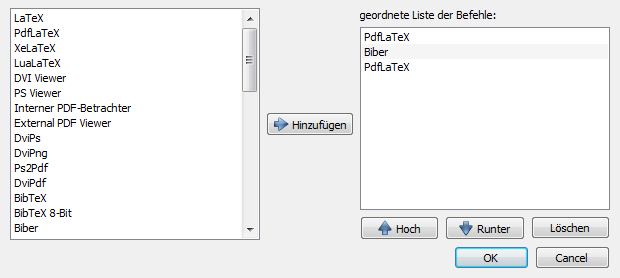
\includegraphics[width=\textwidth]{images/texstudio_optionwindow_build.PNG}
	\caption{Einstellungen für Biber im Optionsfenster}
	\label{figbuildOptions}
\end{figure}


\section{Arara}
arara ist ein TEX-Automatisierungswerkzeug, das auf Regeln und Richtlinien basiert. Es ist in mancher Hinsicht ähnlich wie andere bekannte Tools, wie z.B. latexmk\autocite{latexmk} und rubber\autocite{rubber}. Der Hauptunterschied ist die Tatsache, dass arara auf explizite Anweisungen im Quellcode nachschaut. Durch diese weiß arara was zu tun ist, anstatt sich auf andere Ressourcen, wie z.B. Logfile-Analyse oder MakeFiles zu verlassen. Der Link zum Gihtub Repository ist \url{https://github.com/cereda/arara}. 
%\url{https://texwelt.de/wissen/fragen/8764/was-ist-arara}

Wie schon beschrieben erkennt arara nicht von selbst was es tun soll und ist auf Anweisungen im Quelltext angewiesen. Diese können so aussehen:
\begin{lstlisting}[style=LaTeX]
% arara: pdflatex
% arara: biber
% arara: pdflatex
% arara: pdflatex
\end{lstlisting}

In der Preamble wurden folgende Anweisungen definiert:
\begin{lstlisting}[style=LaTeX]
% arara: pdflatex  { action: nonstopmode, shell: on }
% arara: pdflatex  { action: nonstopmode, shell: on }
% arara: biber
% arara: pdflatex  { action: nonstopmode, shell: on }
% arara: pdflatex  { action: nonstopmode, shell: on }
% arara: clean: { files: [ Index.aux, Index.bbl ] }
% arara: clean: { files: [ Index.bcf, Index.cod ] } 
% arara: clean: { files: [ Index.blg, Index.lof ] }
% arara: clean: { files: [ Index.lot, Index.out ] } 
% arara: clean: { files: [ Index.toc, Index.log ] } 
% arara: clean: { files: [ Index.run.xml ] }
\end{lstlisting}

Die Anweisungen definieren das pdflatex mit den Modi nonstopmode und --shell-escape ausgeführt werden soll. Nach pdflatex wird mit der Anweisung \emph{clean} und der Option \emph{files} noch überflüssigen Dateien entfernt. 
Die Installationsbeschreibung für Windows im Handbuch von arara ist etwas verwirrend, weswegen hier die Installation-Schritte beschrieben werden:
\begin{enumerate}
\item Miktex Update Manager(Admin) starten und aktualisieren lassen
\item Miktex Package Manager starten und dort nachdem Paket arara suchen
\item Paket installieren. (Nutzt nicht in der packages.tex \verb|\usepackage{arara}|)	
\end{enumerate}

Wenn man dann arara noch in TexStudio integrieren möchte sollte man diesen Link aufrufen und lesen. Es funktioniert ähnlich wie, zum Beginn des Kapitels beschrieben, für Biber, nur das man seinen eigenen Prozess definiert. Dazu muss man den Pfad zur Exe kopieren und wie in dem Thread beschrieben wird TexStudio hinzufügen.

Hier der Link: \url{https://tex.stackexchange.com/questions/313616/configuring-arara-in-texstudio-on-windows}

Wenn der Standardcompiler dann auf arara gesetzt wurde drückt man wie gewohnt F5 oder auf den Compiler-Button(Grüner Pfeil).
Für alle die Plots erstellen möchten, ist dies hier ebenfalls interessant: \url{https://latex.org/know-how/435-gnuplot-arara}
Wer Hilfe benötigt beim Einstellen von arara kann auch auf Gitter.im vorbeischauen. Dort gibt es einen Channel indem aktiv geholfen wird. 
\section{LatexMK}
Wie bereits beschrieben reiht sich LatexMK als Automatisierungstool in die Reihe der nützlichen Tools ein. Die Installation von LatexMK erfolgt dabei ebenfalls über den Paket Manager von Miktex oder bei Linux über texlive. Die Handhabung ist hierbei jedoch eine ganz andere als bei \emph{arara}, da dieses Tool keine Anweisungen benötigt. Es kann ebenfalls als Standardcompiler in TexStudio über die bereits beschriebene Methodik festgelegt und kann ebenfalls über die Shell gestartet werden. Hier ein Beispiel: 

\begin{lstlisting}[style=Bash]
$ latexmk -pdf -pv myfile.tex
\end{lstlisting}

Der Vorteil von LatexMK ist, dass es automatisch erkennen kann ob eine Datei verändert wurde. Über die Option \emph{-pv} wird dem Tool mitgeteilt, dass es jedes mal kompilieren soll wenn die Datei verändert wurde. Weitere Erklärungen und Anleitungen findet man hier:
\begin{description}
	\item[Dokumentation: ] \url{http://mg.readthedocs.io/latexmk.html}
	\item[Hauptseite von LatexMK: ] \url{http://personal.psu.edu/jcc8//latexmk/}
	\item[Handbuch des Paketes: ] \url{http://ftp.uni-erlangen.de/ctan/support/latexmk/latexmk.pdf}
\end{description}

\section{Rubber}
Rubber ist ein Programm, dessen Zweck es ist, alle Aufgaben im Zusammenhang mit der Erstellung von LaTeX-Dokumenten zu erledigen. Dazu gehört natürlich auch, das Dokument selbst so oft zu kompilieren, dass alle Referenzen definiert sind. Zur Verwaltung der bibliographischen Referenzen wird BibTeX verwendet. Die automatische Ausführung von dvips zur Erzeugung von PostScript-Dokumenten ist ebenso enthalten wie die Verwendung von pdfLaTeX zur Erzeugung von PDF-Dokumenten. Die Quellenseite von \emph{rubber} ist: \url{https://launchpad.net/rubber} . Das Programm funktioniert wie LatexMK und muss entweder über die Shell genutzt oder wie \emph{arara} in TexStudio als User Command eingebunden werden. Der Aufruf ist ähnlich wie in LatexMK: 

\begin{lstlisting}[style=Bash]
$ rubber --clean --pdf myfile
\end{lstlisting}

In diesem Blog-Eintrag auf Tex-talk.net erklärt der Erfinder von \emph{arara} wie rubber funktioniert: \url{http://tex-talk.net/2011/12/building-documents-with-rubber/} .

	\chapter{Präsentationen erstellen mit \LaTeX}

\url{http://pandoc.org/MANUAL.html#producing-slide-shows-with-pandoc}


	\chapter{Diagramme und Graphen in \LaTeX}
%	\chapter{Schluss}



 
	\newpage

%----------------------------------------------------------------------------------------
%	BIBLIOGRAPHY und Listen
%----------------------------------------------------------------------------------------
	\begin{spacing}{1.0}
		\listoffigures
		\listoftables
		\lstlistoflistings		
		\listofformels
		\nocite{*}
		\printbibliography[title={Literaturverzeichnis}] % If you are writing a german report, you can use [title={Literaturverzeichnis}] insted. 
	\end{spacing}
	\newpage
	
%----------------------------------------------------------------------------------------
%	APPENDIX
%----------------------------------------------------------------------------------------
	\appendix
	\chapter{ToDo Liste}


Weitere Informationen zu Latex
\url{https://github.com/davidstutz/latex-resources}

\end{document}
